\documentclass[a4paper,oneside,english,reqno]{amsbook}
\usepackage[T1]{fontenc}
\synctex=-1
% \usepackage{xcolor}
\usepackage{babel}
\usepackage{textcomp}
\usepackage{mathrsfs}
% \usepackage{url}
\usepackage{amstext}
\usepackage{amsthm}
\usepackage{amssymb}
\usepackage{stmaryrd}
\usepackage{agt}
% \usepackage{rotating}

\makeindex
% \usepackage[all]{xy}
% \usepackage[unicode=true,
%  bookmarks=true,bookmarksnumbered=true,bookmarksopen=false,
%  breaklinks=false,pdfborder={0 0 0},backref=false,colorlinks=true]
%  {hyperref}
\hypersetup{pdftitle={Algebraic General Topology. Volume 1 addons},
 pdfauthor={Victor Porton},
 pdfsubject={general topology},
 pdfkeywords={algebraic general topology,quasi-uniform spaces,generalizations of proximity spaces,generalizations of nearness spaces,generalizations of uniform spaces}}

\usepackage{xr,refcount}
\externaldocument[book-]{book}
\newcommand{\bookref}[1]{\ref*{book-#1}}

% Continue numbering of book.pdf
\setcounter{thm}{\getrefnumber{book-finalthm}}
\addtocounter{thm}{-1}

\global\long\def\Low{\operatorname{Low}}
\global\long\def\Back{\operatorname{Back}}

\begin{document}

\title{Algebraic General Topology. Volume 1 addons}

\author{Victor Porton}

\email{\href{mailto:porton@narod.ru}{porton@narod.ru}}


\urladdr{\href{http://www.mathematics21.org}{http://www.mathematics21.org}}


\date{\today}


\begin{abstract}
This file contains future addons for the free e-book ``Algebraic General
Topology. Volume 1'', which are yet not enough ripe to be included into the
book.
\end{abstract}


\keywords{algebraic general topology, quasi-uniform spaces, generalizations
of proximity spaces, generalizations of nearness spaces, generalizations
of uniform spaces}


\subjclass[2000]{54J05, 54A05, 54D99, 54E05, 54E15, 54E17, 54E99}

\maketitle

\tableofcontents{}

\chapter{About this document}

This file contains future addons for the free e-book ``Algebraic General
Topology. Volume 1'', which are yet not enough ripe to be included into the
book.

Theorem (including propositions, conjectures, etc.) numbers in this document start from the last theorem number
in the book plus one. Theorems references inside this document are hyperlinked, but references
to theorems in the book are not hyperlinked (because PDF viewer Okular 0.20.2 does not support
Backward button after clicking a cross-document reference, and thus I want to avoid clicking such links).

\chapter{Applications of algebraic general topology}

\section{``Hybrid'' objects}

Algebraic general topology allows to construct ``hybrid'' objects of ``continuous'' (as topological spaces)
and discrete (as graphs).

Consider for example $D\sqcup T$ where $D$ is a digraph and $T$ is a topological space.

The $n$-th power $(D\sqcup T)^n$ yields an expression with $2^n$ terms.
So treating $D\sqcup T$ as one object (what becomes possible using algebraic general topology)
rather than the join of two objects may have an exponential benefit for simplicity of formulas.

\section{A way to construct directed topological spaces}

\subsection{Some notation}

I use~$\mathcal{E}$ and $\iota$ notations from {\tt volume-2.pdf}. \fxwarning{Reorder document fragments to describe it before use.}

I remind that $f|_X = f\circ \id_X$ for binary relations, funcoids, and reloid.

$f\parallel_X = f\circ(\mathcal{E}^X)^{-1}$.

$f\square X = \id_X\circ f\circ\id_X^{-1}$.

As proved in {\tt volume-2.pdf}, the following are bijections and moreover isomorphisms (for $R$ being either funcoids or reloids or binary relations):
\begin{enumerate}
\item $\setcond{(f|_X;f\parallel_X)}{f\in R}$;
\item $\setcond{(f\square X;\iota_X f)}{f\in R}$.
\end{enumerate}

As easily follows from these isomorphisms and theorem~\bookref{rect-cont}:

\begin{prop}
For funcoids, reloids, and binary relations:
\begin{enumerate}
\item $f\in\continuous(\mu;\nu)\Rightarrow f\parallel_{A}\in\continuous(\iota_A\mu;\nu)$;
\item $f\in\continuous'(\mu;\nu)\Rightarrow f\parallel_{A}\in\continuous'(\iota_A\mu;\nu)$;
\item $f\in\continuous''(\mu;\nu)\Rightarrow f\parallel_{A}\in\continuous''(\iota_A\mu;\nu)$. 
\end{enumerate}
\end{prop}

\subsection{Directed line and directed intervals}

Let $\mathfrak{A}$ be a poset. We will denote $\overline{\mathfrak{A}}=\mathfrak{A}\cup\{-\infty,+\infty\}$ the poset
with two added elements $-\infty$ and $+\infty$, such that $+\infty$ is strictly greater than every element of~$\mathfrak{A}$
and $-\infty$ is strictly less.

\begin{defn}
For an element~$a$ of a poset~$\mathfrak{A}$
\begin{enumerate}
\item $J_{\geq}(a) = \setcond{x\in\mathfrak{A}}{x\geq a}$;
\item $J_{>}(a) = \setcond{x\in\mathfrak{A}}{x>a}$;
\item $J_{\leq}(a) = \setcond{x\in\mathfrak{A}}{x\leq a}$;
\item $J_{<}(a) = \setcond{x\in\mathfrak{A}}{x<a}$.
\end{enumerate}
\end{defn}

\begin{defn}
Let $a$ be an element of a poset~$\mathfrak{A}$.
\begin{enumerate}
\item $\Delta(a) = \bigsqcap^{\mathscr{F}} \setcond{]x;y[}{x,y\in\overline{\mathfrak{A}}, x<a\land y>a}$;
\item $\Delta_{\geq}(a) = \bigsqcap^{\mathscr{F}} \setcond{[a;y[}{y\in\overline{\mathfrak{A}}, y>a}$;
\item $\Delta_{>}(a) = \bigsqcap^{\mathscr{F}} \setcond{]a;y[}{y\in\overline{\mathfrak{A}}, x<a\land y>a}$;
\item $\Delta_{\leq}(a) = \bigsqcap^{\mathscr{F}} \setcond{]x;a]}{x\in\overline{\mathfrak{A}}, x<a}$.
\item $\Delta_{<}(a) = \bigsqcap^{\mathscr{F}} \setcond{]x;a[}{x\in\overline{\mathfrak{A}}, x<a}$;
\end{enumerate}
\end{defn}

\begin{obvious}
~
\begin{enumerate}
\item $\Delta_{\geq}(a) = \Delta(a)\sqcap^{\mathscr{F}} @J_{\geq a}$;
\item $\Delta_{>}(a) = \Delta(a)\sqcap^{\mathscr{F}} @J_{>a}$;
\item $\Delta_{\leq}(a) = \Delta(a)\sqcap^{\mathscr{F}} @J_{\leq a}$;
\item $\Delta_{<}(a) = \Delta(a)\sqcap^{\mathscr{F}} @J_{<a}$.
\end{enumerate}
\end{obvious}

\begin{defn}
~
Given a partial order~$\mathfrak{A}$ and~$x\in\mathfrak{A}$, the following defines complete funcoids:
\begin{enumerate}
\item $\rsupfun{|\mathfrak{A}|}\{x\} = \Delta(x)$;
\item $\rsupfun{|\mathfrak{A}|_{\geq}}\{x\} = \Delta_{\geq}(x)$;
\item $\rsupfun{|\mathfrak{A}|_{>}}\{x\} = \Delta_{>}(x)$;
\item $\rsupfun{|\mathfrak{A}|_{\leq}}\{x\} = \Delta_{\leq}(x)$;
\item $\rsupfun{|\mathfrak{A}|_{<}}\{x\} = \Delta_{<}(x)$.
\end{enumerate}
\end{defn}

\begin{prop}
The complete funcoid corresponding to the order topology\footnote{See Wikipedia for a definition of ``Order topology''.}
is equal to $|\mathfrak{A}|$.
\end{prop}

\begin{proof}
Because every open set is a finite union of open intervals, the complete funcoid~$f$ corresponding to the order topology
is described by the formula: $\rsupfun{f}\{x\} = \bigsqcap^{\mathscr{F}}\setcond{]a;b[}{a,b\in\overline{\mathfrak{A}}, a<x\land b>x} =
\Delta(x) = \rsupfun{|\mathfrak{A}|}\{x\}$. Thus $f=|\mathfrak{A}|$.
\end{proof}

\begin{xca}
Show that $|\mathfrak{A}|_{\geq}$ (in general) is not the same as ``right order topology''\footnote{See Wikipedia}.
\end{xca}

\begin{prop}
~
\begin{enumerate}
\item $\rsupfun{|\mathfrak{A}|_{\geq}^{-1}}@X = @\setcond{a\in\mathfrak{A}}{\forall y\in\overline{\mathfrak{A}}:(y>a \Rightarrow X\cap[a;y[\ne\emptyset)}$;
\item $\rsupfun{|\mathfrak{A}|_{>}^{-1}}@X = @\setcond{a\in\mathfrak{A}}{\forall y\in\overline{\mathfrak{A}}:(y>a \Rightarrow X\cap]a;y[\ne\emptyset)}$;
\item $\rsupfun{|\mathfrak{A}|_{\leq}^{-1}}@X = @\setcond{a\in\mathfrak{A}}{\forall \in\overline{\mathfrak{A}}:(x<a \Rightarrow X\cap]x;a]\ne\emptyset)}$;
\item $\rsupfun{|\mathfrak{A}|_{<}^{-1}}@X = @\setcond{a\in\mathfrak{A}}{\forall \in\overline{\mathfrak{A}}:(x<a \Rightarrow X\cap]x;a[\ne\emptyset)}$.
\end{enumerate}
\end{prop}

\begin{proof}
$a\in\rsupfun{|\mathfrak{A}|_{\geq}^{-1}}@X \Leftrightarrow
@\{a\} \nasymp \rsupfun{|\mathfrak{A}|_{\geq}^{-1}}@X \Leftrightarrow
\rsupfun{|\mathfrak{A}|_{\geq}}@\{a\} \nasymp @X \Leftrightarrow
\Delta_{\geq}(a) \nasymp @X \Leftrightarrow
\forall y\in\overline{\mathfrak{A}}:(y>a \Rightarrow X\cap[a;y[\ne\emptyset)$.

$a\in\rsupfun{|\mathfrak{A}|_{>}^{-1}}@X \Leftrightarrow
@\{a\} \nasymp \rsupfun{|\mathfrak{A}|_{>}^{-1}}@X \Leftrightarrow
\rsupfun{|\mathfrak{A}|_{>}}@\{a\} \nasymp @X \Leftrightarrow
\Delta_{>}(a) \nasymp @X \Leftrightarrow
\forall y\in\overline{\mathfrak{A}}:(y>a \Rightarrow X\cap]a;y[\ne\emptyset)$.

The rest follows from duality.
\end{proof}

\begin{conjecture}
~
\begin{enumerate}
\item $|\mathbb{R}|_{\geq} = |\mathbb{R}| \sqcap \geq$;
\item $|\mathbb{R}|_{>} = |\mathbb{R}| \sqcap >$;
\item $|\mathbb{R}|_{\leq} = |\mathbb{R}| \sqcap \leq$;
\item $|\mathbb{R}|_{<} = |\mathbb{R}| \sqcap <$.
\end{enumerate}
\end{conjecture}

\begin{rem}
On trivial ultrafilters these obviously agree:
\begin{enumerate}
\item $\rsupfun{|\mathbb{R}|_{\geq}}\{x\} = \rsupfun{|\mathbb{R}| \sqcap \geq}\{x\}$;
\item $\rsupfun{|\mathbb{R}|_{>}}\{x\} = \rsupfun{|\mathbb{R}| \sqcap >}\{x\}$;
\item $\rsupfun{|\mathbb{R}|_{\leq}}\{x\} = \rsupfun{|\mathbb{R}| \sqcap \leq}\{x\}$;
\item $\rsupfun{|\mathbb{R}|_{<}}\{x\} = \rsupfun{|\mathbb{R}| \sqcap <}\{x\}$.
\end{enumerate}
\end{rem}

I will say that a property holds on a filter~$\mathcal{A}$ iff there is $A\in\up\mathcal{A}$ on which the property holds.

\fxnote{$f\in\continuous(A;B)\land f\in\continuous(\iota_A|\mathbb{R}|_{\geq};\iota_B|\mathbb{R}|_{\geq}) \Leftrightarrow
(f;f)\in\continuous((A;\iota_A|\mathbb{R}|_{\geq});(B;\iota_B|\mathbb{R}|_{\geq}))$}

\begin{lem}
Let function~$f:A\rightarrow B$ where $A,B\in\subsets\mathbb{R}$ and $A$ is connected.
\begin{enumerate}
\item $f$ is monotone and $f\in\continuous(A;B)$ iff
$f\in\continuous(A;B)\cap\continuous(\iota_A|\mathbb{R}|_{\geq};\iota_B|\mathbb{R}|_{\geq})$ iff
$f\in\continuous(A;B)\cap\continuous(\iota_A|\mathbb{R}|_{>};\iota_B|\mathbb{R}|_{\geq})$ iff
$f\in\continuous(\iota_A|\mathbb{R}|_{\geq};\iota_B|\mathbb{R}|_{\geq})\cap
\continuous(\iota_A|\mathbb{R}|_{\leq};\iota_B|\mathbb{R}|_{\leq})$.
\item $f$ is strictly monotone and $\in\continuous(A;B)$ iff
$f\in\continuous(A;B)\cap\continuous(\iota_A|\mathbb{R}|_{>};\iota_B|\mathbb{R}|_{>})$ iff
$f\in\continuous(\iota_A|\mathbb{R}|_{>};\iota_B|\mathbb{R}|_{>})\cap
\continuous(\iota_A|\mathbb{R}|_{<};\iota_B|\mathbb{R}|_{<})$.
\end{enumerate}
\fxnote{It is equivalent to
\[
(\mylambda{t}{\mathbb{R}}{f(x+t)})|_{\Delta}\sqsubseteq
(\Delta_{\leq}\times^{\mathsf{FCD}}\Delta_{\leq}(f(x)))\sqcup(\Delta_{\geq}\times^{\mathsf{FCD}}\Delta_{\geq}(f(x)))).
\]}
\fxnote{Generalize for arbitrary posets.}
\fxnote{Generalize for $f$ being a funcoid.}
\end{lem}

\begin{proof}
Because $f$ is continuous, we have $\rsupfun{f\circ\iota_A|\mathbb{R}|}\{x\} \sqsubseteq \rsupfun{\iota_B|\mathbb{R}|\circ f}\{x\}$
that is $\rsupfun{f} \Delta(x) \sqsubseteq \Delta(f(x))$ for every~$x$.

If $f$ is monotone, we have $\rsupfun{f} \Delta_{\geq}(x) \sqsubseteq [f(x);\infty[$.
Thus $\rsupfun{f} \Delta_{\geq}(x) \sqsubseteq \Delta_{\geq}(f(x))$, that is
$\rsupfun{f\circ \iota_A|\mathbb{R}|_{\geq}}\{x\} \sqsubseteq \rsupfun{\iota_B|\mathbb{R}|_{\geq}\circ f}\{x\}$, thus
$f\in\continuous(\iota_A|\mathbb{R}|_{\geq};\iota_B|\mathbb{R}|_{\geq})$.

If $f$ is strictly monotone, we have $\rsupfun{f} \Delta_{>}(x) \sqsubseteq ]f(x);\infty[$.
Thus $\rsupfun{f} \Delta_{>}(x) \sqsubseteq \Delta_{>}(f(x))$, that is
$\rsupfun{f\circ \iota_A|\mathbb{R}|_{>}}\{x\} \sqsubseteq \rsupfun{\iota_B|\mathbb{R}|_{>}\circ f}\{x\}$, thus
$f\in\continuous(\iota_A|\mathbb{R}|_{>};\iota_B|\mathbb{R}|_{>})$.

Let now $f\in\continuous(\iota_A|\mathbb{R}|_{\geq};\iota_B|\mathbb{R}|_{\geq})$.

Take any~$a\in A$ and let $c=\setcond{b\in B}{b\geq a, \forall x\in[a;b[: f(x)\geq f(a)}$.
It's enough to prove that $c$ is the right endpoint (finite or infinite) of~$A$.

Indeed by continuity $f(a)\leq f(c)$ and if $c$ is not already the right endpoint of~$A$, then
there is $b'>c$ such that $\forall x\in[c;b'[: f(x)\geq f(c)$.
So we have $\forall x\in[a;b'[: f(x)\geq f(c)$ what contradicts to the above.

So $f$ is monotone on the entire~$A$.

$f\in\continuous(\iota_A|\mathbb{R}|_{\geq};\iota_B|\mathbb{R}|_{\geq}) \Rightarrow f\in\continuous(\iota_A|\mathbb{R}|_{>};\iota_B|\mathbb{R}|_{\geq})$ is obvious. Reversely
$f\in\continuous(\iota_A|\mathbb{R}|_{>};\iota_B|\mathbb{R}|_{\geq}) \Rightarrow
f\circ \iota_A|\mathbb{R}|_{>} \sqsubseteq \iota_B|\mathbb{R}|_{\geq}\circ f \Leftrightarrow
\forall x\in\mathbb{R}: \supfun{f}\rsupfun{\iota_A|\mathbb{R}|_{>}}\{x\} \sqsubseteq \rsupfun{\iota_B|\mathbb{R}|_{\geq}}\rsupfun{f}\{x\} \Leftrightarrow
\forall x\in\mathbb{R}: \supfun{f}\Delta_{>}(x) \sqsubseteq \Delta_{\geq}f(x) \Leftrightarrow
\forall x\in\mathbb{R}: \supfun{f}\Delta_{>}(x) \sqcup \{f(x)\} \sqsubseteq \Delta_{\geq}f(x) \Leftrightarrow
\forall x\in\mathbb{R}: \supfun{f}\Delta_{>}(x) \sqcup \{x\} \sqsubseteq \Delta_{\geq}f(x) \Leftrightarrow
\forall x\in\mathbb{R}: \supfun{f}\Delta_{\geq}(x) \sqsubseteq \Delta_{\geq}f(x) \Leftrightarrow
\forall x\in\mathbb{R}: \supfun{f}\rsupfun{\iota_A|\mathbb{R}|_{\geq}}\{x\} \sqsubseteq \rsupfun{\iota_B|\mathbb{R}|_{\geq}}\rsupfun{f}\{x\} \Leftrightarrow
\forall x\in\mathbb{R}: f\circ \iota_A|\mathbb{R}|_{\geq} \sqsubseteq \iota_B|\mathbb{R}|_{\geq}\circ f \Leftrightarrow
f\in\continuous(\iota_A|\mathbb{R}|_{\geq};\iota_B|\mathbb{R}|_{\geq})$.

Let $f\in\continuous(\iota_A|\mathbb{R}|_{>};\iota_B|\mathbb{R}|_{>})$. Then $f\in\continuous(\iota_A|\mathbb{R}|_{>};\iota_B|\mathbb{R}|_{\geq})$ and thus it is monotone.
We need to prove that $f$ is strictly monotone.
Suppose the contrary. Then there is a nonempty interval $[p;q]\subseteq A$ such that $f$ is constant on this interval.
But this is impossible because $f\in\continuous(\iota_A|\mathbb{R}|_{>};\iota_B|\mathbb{R}|_{>})$.

Prove that $f\in\continuous(\iota_A|\mathbb{R}|_{\geq};\iota_B|\mathbb{R}|_{\geq})\cap
\continuous(\iota_A|\mathbb{R}|_{\leq};\iota_B|\mathbb{R}|_{\leq})$ implies
$f\in\continuous(A;B)$. Really, it implies
$\supfun{f}\Delta_{\leq}(x)\sqsubseteq\Delta_{\leq}(fx)$ and $\supfun{f}\Delta_{\geq}(x)\sqsubseteq\Delta_{\geq}(fx)$
thus $\supfun{f}\Delta(x) = \supfun{f}(\Delta_{\leq}(x)\sqcup\{x\}\sqcup\Delta_{\geq}(x)) \subseteq
\Delta_{\leq}f(x)\sqcup\{f(x)\}\sqcup\Delta_{\geq}f(x) =
\Delta(f(x))$.

Prove that $f\in\continuous(\iota_A|\mathbb{R}|_{>};\iota_B|\mathbb{R}|_{>})\cap
\continuous(\iota_A|\mathbb{R}|_{<};\iota_B|\mathbb{R}|_{<})$
$f\in\continuous(A;B)$. Really, it implies
$\supfun{f}\Delta_{<}(x)\sqsubseteq\Delta_{<}(fx)$ and $\supfun{f}\Delta_{>}(x)\sqsubseteq\Delta_{>}(fx)$
thus $\supfun{f}\Delta(x) = \supfun{f}(\Delta_{<}(x)\sqcup\{x\}\sqcup\Delta_{>}(x)) \subseteq
\Delta_{<}f(x)\sqcup\{f(x)\}\sqcup\Delta_{>}f(x) = \Delta(f(x))$.
\end{proof}

\begin{thm}
Let function~$f:A\rightarrow B$ where $A,B\in\subsets\mathbb{R}$.
\begin{enumerate}
\item $f$ is locally monotone and $f\in\continuous(A;B)$ iff
$f\in\continuous(A;B)\cap\continuous(\iota_A|\mathbb{R}|_{\geq};\iota_B|\mathbb{R}|_{\geq})$ iff
$f\in\continuous(A;B)\cap\continuous(\iota_A|\mathbb{R}|_{>};\iota_B|\mathbb{R}|_{\geq})$ iff
$f\in\continuous(\iota_A|\mathbb{R}|_{\geq};\iota_B|\mathbb{R}|_{\geq})\cap
\continuous(\iota_A|\mathbb{R}|_{\leq};\iota_B|\mathbb{R}|_{\leq})$.
\item $f$ is locally strictly monotone and $\in\continuous(A;B)$ iff
$f\in\continuous(A;B)\cap\continuous(\iota_A|\mathbb{R}|_{>};\iota_B|\mathbb{R}|_{>})$ iff
$f\in\continuous(\iota_A|\mathbb{R}|_{>};\iota_B|\mathbb{R}|_{>})\cap
\continuous(\iota_A|\mathbb{R}|_{<};\iota_B|\mathbb{R}|_{<})$.
\end{enumerate}
\end{thm}

\begin{proof}
By the lemma it is (strictly) monotone on each connected component.
\end{proof}

See also related math.SE questions:
\begin{enumerate}
\item \url{http://math.stackexchange.com/q/1473668/4876}
\item \url{http://math.stackexchange.com/a/1872906/4876}
\item \url{http://math.stackexchange.com/q/1875975/4876}
\end{enumerate}

\subsection{Directed topological spaces}

Directed topological spaces are defined at\\
\url{http://ncatlab.org/nlab/show/directed+topological+space}

\begin{defn}
A \emph{directed topological space} (or \emph{d-space} for short) is a pair $(X;d)$ of a topological space~$X$ and
a set $d\subseteq\continuous([0;1];X)$ (called \emph{directed paths} or \emph{d-paths}) of paths in~$X$ such that
\begin{enumerate}
\item (constant paths) every constant map $[0;1]\to X$ is directed;
\item (reparameterization) $d$ is closed under composition with increasing continuous maps $[0;1]\to [0;1]$;
\item (concatenation) $d$ is closed under path-concatenation: if the d-paths $a$, $b$ are consecutive in $X$ ($a(1)=b(0)$), then their ordinary concatenation $a+b$ is also a d-path
\begin{gather*}
(a+b)(t) = a(2t),\,\text{if}\, 0\le t\le \frac{1}{2}, \\
(a+b)(t) = b(2t-1),\,\text{if}\, \frac{1}{2}\le t\le 1.
\end{gather*}
\end{enumerate}
\end{defn}

I propose a new way to construct a directed topological space. My way is more geometric/topological as it does not involve dealing with particular paths.

\begin{defn}
Let $ T$ be the complete endofuncoid corresponding to a topological space
and $\nu\sqsubseteq T$ be its ``subfuncoid''. The $\mathrm{d}$-space $\operatorname{(dir)}(T;\nu)$ induced by the pair $(T;\nu)$
consists of~$ T$ and paths $f\in\continuous([0;1]; T) \cap \continuous(|[0;1]|_{\geq}; \nu)$
such that $f(0)=f(1)$.
\end{defn}

\begin{prop}
It is really a $\mathrm{d}$-space.
\end{prop}

\begin{proof}
Every $\mathrm{d}$-path is continuous.

Constant path are $\mathrm{d}$-paths because $\nu$ is reflexive.

Every reparameterization is a $\mathrm{d}$-path because they are $\continuous(|[0;1]|_{\geq}; \nu)$ and we can apply the theorem about
composition of continuous functions.

Every concatenation is a $\mathrm{d}$-path. Denote
$f_0 = \mylambda{t}{[0;\frac{1}{2}]}{a(2t)}$ and $f_1 = \mylambda{t}{[\frac{1}{2};1]}{b(2t-1)}$.
Obviously $f_0,f_1 \in \continuous([0;1];\mu) \cap \continuous(|[0;1]|_{\geq}; \nu)$.
Then we conclude that $a+b = f_1\sqcup f_1$ is in $f_0,f_1 \in \continuous([0;1];\mu) \cap \continuous(|[0;1]|_{\geq}; \nu)$
using the fact that the operation $\circ$ is distributive over $\sqcup$.
\end{proof}

Below we show that not every $\mathrm{d}$-space is induced by a pair of an endofuncoid and its subfuncoid.
But are $\mathrm{d}$-spaces not represented this way good anything except counterexamples?

Let now we have a $\mathrm{d}$-space $(X;d)$. Define funcoid~$\nu$ corresponding to the $\mathrm{d}$-space by the formula
$\nu = \bigsqcup_{a\in d}(a\circ |\mathbb{R}|_{\geq}\circ a^{-1})$.

\begin{example}
The two directed topological spaces, constructed from a fixed topological space and two different reflexive funcoids,
are the same.
\end{example}

\begin{proof}
Consider the indiscrete topology~$T$ on $\mathbb{R}$ and the funcoids~$1^{\mathsf{FCD}(\mathbb{R};\mathbb{R})}$
and $1^{\mathsf{FCD}(\mathbb{R};\mathbb{R})}\sqcup(\{0\}\times^{\mathsf{FCD}} \Delta_{\geq})$.
The only $\mathrm{d}$-paths in both these settings are constant functions.
\end{proof}

\begin{example}
A $\mathrm{d}$-space is not determined by the induced funcoid.
\end{example}

\begin{proof}
The following a $\mathrm{d}$-space induces the same funcoid as the $\mathrm{d}$-space of all paths on the plane.

Consider a plane $\mathbb{R}^2$ with the usual topology. Let $\mathrm{d}$-paths be paths lying inside a polygonal chain (in the plane).
\end{proof}

\begin{conjecture}
A $\mathrm{d}$-path~$a$ is determined by the funcoids (where $x$ spans $[0;1]$)
\[ (\mylambda{t}{\mathbb{R}}{a(x+t)})|_{\Delta(0)}. \]
\end{conjecture}

\section{A way to construct directed topological spaces}

\fxnote{Should include definition of directed topological space.}

Directed topological spaces are defined at\\
\url{http://ncatlab.org/nlab/show/directed+topological+space}

I propose a new way to construct a directed topological space. My way is more geometric/topological as it does not involve dealing with particular paths.

\begin{conjecture}
Every directed topological space can be constructed in the below described way.
\end{conjecture}

Consider topological space $T$ and its subfuncoid $F$ (that is $F$ is a funcoid which is less that $T$ in the order of funcoids).
Note that in our consideration $F$ is an endofuncoid (its source and destination are the same).

Then a directed path from point $A$ to point $B$ is defined as a continuous function $f$ from $[0;1]$ to $F$ such that $f(0)=A$ and $f(1)=B$.
\fxwarning{Specify whether the interval $[0;1]$ is treated as a proximity, pretopology, or preclosure.}

Because $F$ is less that $T$, we have that every directed path is a path.

\begin{conjecture}
The two directed topological spaces, constructed from a fixed topological space and two different funcoids,
are different.
\end{conjecture}

For a counter-example of (which of the two?) the conjecture consider funcoid $T\sqcap(\mathbb{Q}\times^{\mathsf{FCD}}\mathbb{Q})$
where $T$ is the usual topology on real line.We need to consider stability of existence and uniqueness of a path under transformations of our funcoid and
under transformations of the vector field. Can this be a step to solve Navier-Stokes existence and smoothness problems?

\section{Integral curves}

\fxwarning{This section is a very rough draft.}

See also \url{https://en.wikipedia.org/wiki/Slope_field}

Let $d$ be a vector field in~$\mathbb{R}^n$ (for a finite~$n$).

\fxnote{$\mathbb{R}$ is made into a ``locally ordered'' space by a direction field. Then use properties of ordered spaces to define the funcoid.}

\begin{defn}
\emph{Integral curve} is a function $f:[0;1]\rightarrow\mathbb{R}^n$ such that $f'(t)=d(f(t))$ for every $t\in[0;1]$.
\end{defn}

\begin{defn}
The definition of \emph{right side integral curve} is the above definition with right derivative of~$f$ instead of derivative~$f'$.
\emph{Left side integral curve} is defined similarly.
\end{defn}

$R(d;\phi) = \setcond{v\in\mathbb{R}^n}{\widehat{vd}<\phi, v\ne 0}$ for $d\ne 0$ and $R(d;\phi) = 0$ if $d=0$,
where $\widehat{ab}$ is the angle between the vectors $a$ and $b$,
for a direction~$d$ and an angle~$\phi$.

$W(d) = \bigsqcap^{\mathsf{RLD}}\setcond{R(d;\phi)}{\phi\in\mathbb{R},\phi>0} \sqcap \Delta^{(\mathsf{RLD})n}$
where \[ \Delta^{(\mathsf{RLD})n} = \underbrace{\Delta\times^{\mathsf{RLD}}\dots\times^{\mathsf{RLD}}\Delta}_{n\text{ times}}. \]
\fxnote{Consider also $\mathsf{FCD}$ instead of $\mathsf{RLD}$. This would use pointfree funcoids.}

Finally our funcoids are the complete funcoid~$Q_+$ and~$Q_-$ described by the formulas
\[
\rsupfun{Q_+}@\{p\} = \supfun{p+} W(d(p)) \quad\text{and}\quad \rsupfun{Q_-}@\{p\} = \supfun{p+} W(-d(p)).
\]
Here $\Delta$ is taken from the ``counter-examples'' section.

In other words,
\[
Q_+ = \bigsqcup_{p\in\mathbb{R}} (@\{p\}\times^{\mathsf{FCD}}\supfun{p+}{W(d(p))});
\quad
Q_- = \bigsqcup_{p\in\mathbb{R}} (@\{p\}\times^{\mathsf{FCD}}\supfun{p+}{W(-d(p))}).
\]

\fxnote{Describe the co-complete funcoids reverse to these complete funcoids.}

\begin{thm}
$f$ is an image of integral curve for a direction field~$d$ iff
$f\in\continuous(|\mathbb{R}|_{>};Q_+)\cap\continuous(|\mathbb{R}|_{<};Q_-)$.
\fxnote{Generalize for subsets of real numbers.}
\end{thm}

\begin{proof}
Equivalently transform $f\in\continuous(\iota_{[0;1]}|\mathbb{R}|;Q)$; $f\circ \iota_{[0;1]}|\mathbb{R}|\sqsubseteq Q\circ f$;
$\rsupfun{f\circ \iota_{[0;1]}|\mathbb{R}|}@\{t\}\sqsubseteq \rsupfun{Q\circ f}@\{t\}$;
$\rsupfun{f}\Delta_{>}(t)\sqcap[0;1])\sqsubseteq \rsupfun{Q}f(t)$;
$\rsupfun{f}\Delta_{>}(t)\sqsubseteq \rsupfun{Q}f(t)$;
$\rsupfun{f}\Delta_{>}(t)\sqsubseteq f(t)+W(D(f(t)))$;
$\rsupfun{f}\Delta_{>}(t)-f(t)\sqsubseteq W(D(f(t)))$;
\[ \forall r>0, \phi>0 \exists\delta>0: \rsupfun{f}(]t;t+\delta[)-f(t)\subseteq R(d;\phi) \cap B_r(f(t)) \]
\[ \forall r>0, \phi>0 \exists\delta>0: \frac{\rsupfun{f}(]t;t+\delta[)-f(t)}{\delta}\subseteq R(d;\phi) \cap B_{r/\delta}(f(t)) \]
??
\end{proof}

\fxnote{The condition that left and right derivatives are the same is equal to continuity in $\mathbb{R}^{n+1}$.}

Explicitly construct this funcoid as (now, for simplicity only for $\mathbb{R}^n$, there is only one direction $d(p)$ per point~$p$):

Alternatively consider $G(p) = \Delta_+\times^{\mathsf{RLD}}Q_+(p) \sqcup \Delta_-\times^{\mathsf{RLD}}Q_-(p)$.
\[ (\mylambda{t}{\mathbb{R}}{f(x+t)-f(x)})|_{\Delta} \sqsubseteq G(x). \]

\begin{conjecture}
If the curve goes only through points with exactly one direction, then the curve is smooth (if it is continuous regarding the above funcoid).
\end{conjecture}

\fxnote{This probably can be generalized for $C^n$ and $C^\infty$ curves. Consider also fractional~$n$. What about curves limited by an exponent?}

$f'(t)=d(f(t))$ is equivalent to $w(x,t)=(v(x),t)$ being a continuous function on~$\mathbb{R}^{n+1}$ with direction specified by
$F(v(t), 1)$.

\subsection{Plural funcoids}

Take $I_+$ and $Q_+$ as described above in forward direction and $I_-$ and $Q_-$ in backward direction. Then
\[ f\in\continuous(I_+;Q_+)\land f\in\continuous(I_-;Q_-) \Leftrightarrow f\times f\in\continuous(I_+\times^{(A)}I_-;Q_+\times^{(A)}Q_-)? \]

To describe the above we can introduce new term \emph{plural funcoids}. This is simply a map
from an index set to funcoids. Composition is defined component-wise. Order is defined as product order.
Well, do we need this? Isn't it the same as infimum product of funcoids?

\subsection{Multiple allowed directions per point}

\[ \rsupfun{Q}@\{p\} = \bigsqcup_{d\in d(p)} \supfun{p+} W(d). \]

One advantage to use funcoids in this case, that when describing the curves we don't need to require that the curve is smooth. I think, it's a big advantage.

It seems (check!) that solutions not only of differential equations but also of difference equations can be
expressed as paths in funcoids.
\chapter{Generalized cofinite filters}

The following is a straightforward generalization of cofinite filter.

\begin{defn}
  $\Omega_{1 a} = \bigsqcap^{\mathfrak{A}}_{X \in
  \operatorname{coatoms}^{\mathfrak{Z}}} X$; $\Omega_{1 b} =
  \bigsqcap^{\mathfrak{A}}_{X \in \operatorname{coatoms}^{\mathfrak{A}}} X$.
\end{defn}

\begin{prop}
The following is an implications tuple:
\begin{enumerate}
 \item\label{omeq-pow} $(\mathfrak{A},\mathfrak{Z})$ is a powerset filtrator.
 \item\label{omeq-flt} $(\mathfrak{A},\mathfrak{Z})$ is a primary filtrator.
 \item\label{omeq-res} $\Omega_{1 a} = \Omega_{1 b}$ for this filtrator.
\end{enumerate}  
\end{prop}

\begin{proof}
~
\begin{description}
 \item[\ref{omeq-pow}$\Rightarrow$\ref{omeq-flt}] Obvious.
 \item[\ref{omeq-flt}$\Rightarrow$\ref{omeq-res}] Proposition 531.
\end{description}
\end{proof}

\begin{prop}
  Let $(\mathfrak{A},\mathfrak{Z})$ be a primary filtrator.
  Let $\mathfrak{Z}$ be a subset of $\subsets U$. Let it be a
  meet-semilattice with greatest element.
  Let also every non-coempty cofinite set lies in
  $\mathfrak{Z}$. Then
  \begin{equation}
    \corestar \Omega = \setcond{ Y \in \mathfrak{Z} }{
    \card \atoms^{\mathfrak{Z}} Y \geq \omega } .
    \label{d-cofin}
  \end{equation}
\end{prop}

\begin{proof}
  $\Omega$ exists by corollary~\bookref{filt-is-complete}.
  
  $Y \in \corestar \Omega \Leftrightarrow Y \nasymp^{\mathfrak{A}} 
  \bigsqcap^{\mathfrak{A}}_{X \in \operatorname{coatoms}^{\mathfrak{Z}}} X
  \Leftrightarrow \text{(by properties of filter bases)} \Leftrightarrow
  \forall S \in \subsets_{\operatorname{fin}} \operatorname{coatoms}^{\mathfrak{Z}} : Y
  \nasymp^{\mathfrak{A}} \bigsqcap^{\mathfrak{A}} S \Leftrightarrow
  \text{(theorem~\bookref{f-meet-closed})} \Leftrightarrow \forall S \in \subsets_{\operatorname{fin}}
  \operatorname{coatoms}^{\mathfrak{Z}} : Y \nasymp \bigsqcap S \Leftrightarrow
  \forall K \in \subsets_{\operatorname{fin}} U : Y \setminus K \neq \emptyset
  \Leftrightarrow \card Y \geq \omega \Leftrightarrow \card
  \atoms^{\mathfrak{Z}} Y \geq \omega$.
  \fxwarning{Define $\subsets_{\operatorname{fin}}$.}
\end{proof}

\begin{cor}
  Formula (\ref{d-cofin}) holds for both reloids and funcoids.
\end{cor}

\begin{proof}
  For reloiods it's straightforward, for funcoids take that they are
  isomorphic to filters on lattice $\Gamma$.
\end{proof}

\begin{cor}
$\Omega^{\mathsf{FCD}} \ne \bot^{\mathsf{FCD}}$ (for $\mathsf{FCD}(A,B)$ where $A\times B$ is an infinite set).
\end{cor}

\begin{prop}\label{omega-bot}
The following is an implications tuple:
\begin{enumerate}
 \item\label{omega-bot-pow} $(\mathfrak{A},\mathfrak{Z})$
  is a powerset filtrator.
 \item\label{omega-bot-flt} $(\mathfrak{A},\mathfrak{Z})$
   is a primary filtrator over an atomic ideal base
   and   $\forall \alpha \in
  \atoms^{\mathfrak{Z}} \exists X \in \up \Omega_{1 a} : a
  \nsqsubseteq X$.
 \item\label{omega-bot-cond} $\Omega_{1 a}$ and $\Cor \Omega_{1 a}$ are defined,
  $\forall \alpha \in
  \atoms^{\mathfrak{Z}} \exists X \in \up \Omega_{1 a} : a
  \nsqsubseteq X$ and $\mathfrak{Z}$ is an atomic poset.
 \item\label{omega-bot-res} $\Cor \Omega_{1 a} = \bot^{\mathfrak{Z}}$.
\end{enumerate}  
\end{prop}

\begin{proof}
~
\begin{description}
\item[\ref{omega-bot-pow}$\Rightarrow$\ref{omega-bot-flt}]
  Obvious.
\item[\ref{omega-bot-flt}$\Rightarrow$\ref{omega-bot-cond}]
  Obvious.
\item[\ref{omega-bot-cond}$\Rightarrow$\ref{omega-bot-res}]
  Suppose $\alpha \in \atoms^{\mathfrak{Z}} \Cor \Omega$. Then
  $\exists X \in \up \Omega : \alpha \nsqsubseteq X$.
  Therefore $\alpha \notin \Cor \Omega$. So $\atoms^{\mathfrak{Z}}
  \Cor \Omega_{1 a} = \emptyset$ and thus by atomicity $\Cor
  \Omega_{1 a} = \bot^{\mathfrak{Z}}$.
\end{description}
\end{proof}

\begin{cor}
  $\Cor \Omega^{\mathsf{FCD}} = \bot$.
\end{cor}

\begin{prop}
  $\Omega_{1 a} = \max \setcond{ \mathcal{X} \in \mathfrak{A} }{
  \Cor \mathcal{X} = \bot^{\mathfrak{Z}} }$ if $\mathfrak{A}$ is
  a complete lattice,
  $\forall \alpha \in \atoms^{\mathfrak{Z}} \exists X \in \up
  \Omega : a \nsqsubseteq X$ and $\mathfrak{Z}$ is an atomic
  poset and $(\mathfrak{A}; \mathfrak{Z})$ is a filtered filtrator.
\end{prop}

\begin{proof}
  Due the last proposition, it is enough to show that $\Cor \mathcal{X}
  = \bot^{\mathfrak{Z}} \Rightarrow \mathcal{X} \sqsubseteq \Omega_{1 a}$ for
  every $\mathcal{X} \in \mathfrak{A}$.
  
  Let $\Cor \mathcal{X} = \bot^{\mathfrak{Z}}$ for some $\mathcal{X} \in
  \mathfrak{A}$. Because of our filtrator being filtered, it's enough to show
  $X \in \up \Omega_{1 a}$. $X = a_0 \sqcap \ldots \sqcap a_n$ for $a_i$
  being coatoms of $\mathfrak{Z}$. $a_i \sqsupseteq \mathcal{X}$ because
  otherwise $a_i \nsqsupseteq \Cor \mathcal{X}$. So $X
  \in \up \Omega_{1 a}$.
\end{proof}

\begin{prop}
  $\up \Omega_{1a} = \setcond{ \bigsqcap S }{ S \in
  \subsets_{\operatorname{fin}} \operatorname{coatoms}^{\mathfrak{Z}} }$
  if it is defined.
\end{prop}

\begin{proof}
  Because $\setcond{ \bigsqcap S }{ S \in
  \subsets_{\operatorname{fin}} \operatorname{coatoms}^{\mathfrak{Z}} }$ is a
  filter.
\end{proof}

\begin{cor}
  $\up \Omega^{\mathsf{FCD}} = \up
  \Omega^{\mathsf{RLD}}$.
\end{cor}

\begin{defn}
$\Omega_{1c} =
\bigsqcup(\atoms^{\mathfrak{A}}\setminus\mathfrak{Z})$.
\end{defn}

\begin{prop}
$\Omega_{1c} = \Omega_{1a}$ provided
  $\forall \alpha \in \atoms^{\mathfrak{Z}} \exists X \in \up
  \Omega : a \nsqsubseteq X$ and $\mathfrak{Z}$ is an atomic
  poset and $(\mathfrak{A}; \mathfrak{Z})$ is a down-aligned
  filtered filtrator and $\mathfrak{Z}$ is atomistic and~$\mathfrak{A}$
  is a complete lattice.
\end{prop}

\begin{proof}
For $x\in\atoms^{\mathfrak{A}}\setminus\mathfrak{Z}$ we have
$\Cor x=\bot$ because otherwise $\bot\ne\Cor x\sqsubset x$.
Thus by previous $x\sqsubseteq\Omega_{1a}$ and so
$\Omega_{1c} =
\bigsqcup(\atoms^{\mathfrak{A}}\setminus\mathfrak{Z}) \sqsubseteq
\Omega_{1a}$.

If $x\in\atoms\Omega_{1a}$ then $x\notin\mathfrak{Z}$ because otherwise
$\Cor x\ne\bot$. So \[ \Omega_{1a}=\bigsqcup\atoms \Omega_{1a}=
\bigsqcup(\atoms \Omega_{1a}\setminus\mathfrak{Z})\sqsubseteq
\bigsqcup(\atoms^{\mathfrak{A}}\setminus\mathfrak{Z}) =
\Omega_{1c}. \]
\end{proof}

\fxnote{Above should be made into an implications tuple (also
above).}

\begin{thm}
The following is an implications tuple:
\begin{enumerate}
\item\label{cor-adj-omega-pow}
  $(\mathfrak{A},\mathfrak{Z})$ is a powerset filtrator.
\item\label{cor-adj-omega-cond}
  $(\mathfrak{A},\mathfrak{Z})$ is a primary filtrator over
  a complete atomic boolean lattice.
\item\label{cor-adj-omega-flt} All of the following:
  \begin{enumerate}
    \item $\mathfrak{A}$ is atomistic complete starrish lattice.
    \item $\mathfrak{Z}$ is a complete atomistic lattice.
    \item $(\mathfrak{A},\mathfrak{Z})$ is a filtered
      down-aligned filtrator with binarily meet-closed core.
  \end{enumerate}
\item\label{cor-adj-omega-res} $\Cor'$ is the lower adjoint of
  $\Omega_{1c}\sqcup^{\mathfrak{A}}-$.
\end{enumerate}
\end{thm}

\begin{proof}
~
\begin{widedisorder}
\item[\ref{cor-adj-omega-pow}$\Rightarrow$\ref{cor-adj-omega-cond}]
Obvious.

\item[\ref{cor-adj-omega-cond}$\Rightarrow$\ref{cor-adj-omega-flt}]
Obvious.

\item[\ref{cor-adj-omega-flt}$\Rightarrow$\ref{cor-adj-omega-res}]
It with join-closed core by theorem~\bookref{semifilt-joinclosed}.

We will prove $\Cor'\mathcal{X} \sqsubseteq \mathcal{Y} \Leftrightarrow
\mathcal{X} \sqsubseteq \Omega_{1c} \sqcup \mathcal{Y}$.

By atomisticity it is equivalent to:
$\atoms^{\mathfrak{A}}\Cor'\mathcal{X} \subseteq \atoms^{\mathfrak{A}}\mathcal{Y}
\Leftrightarrow
\atoms^{\mathfrak{A}}\mathcal{X} \subseteq \atoms^{\mathfrak{A}}(\Omega_{1c} \sqcup \mathcal{Y})$;
(theorem~\bookref{dual-core-join})
$\atoms^{\mathfrak{A}}\Cor'\mathcal{X} \subseteq \atoms^{\mathfrak{A}}\mathcal{Y}
\Leftrightarrow
\atoms^{\mathfrak{A}}\mathcal{X} \subseteq \atoms^{\mathfrak{A}}\Omega_{1c} \cup \atoms^{\mathfrak{A}}\mathcal{Y}$;
what by below is equivalent to:
$\atoms^{\mathfrak{Z}}  \mathcal{X} \subseteq
\atoms^{\mathfrak{Z}}  \mathcal{Y} \Leftrightarrow
\atoms^{\mathfrak{A}}  \mathcal{X} \subseteq \atoms^{\mathfrak{A}}
\Omega_{1c} \cup \atoms^{\mathfrak{A}}  \mathcal{Y}$.

$\Cor' \mathcal{X} \sqsubseteq \mathcal{Y} \Leftrightarrow
\atoms^{\mathfrak{A}} \Cor' \mathcal{X} \subseteq
\atoms^{\mathfrak{A}}  \mathcal{Y} \Rightarrow
\atoms^{\mathfrak{Z}} \Cor' \mathcal{X} \subseteq
\atoms^{\mathfrak{Z}}  \mathcal{Y} \Leftrightarrow
\atoms^{\mathfrak{Z}}  \mathcal{X} \subseteq \atoms^{\mathfrak{Z}}
\mathcal{Y}$;

$\atoms^{\mathfrak{Z}}  \mathcal{X} \subseteq
\atoms^{\mathfrak{Z}}  \mathcal{Y} \Rightarrow
\text{(theorem~\bookref{cor-join-atom})} \Rightarrow
\Cor' \mathcal{X}
\sqsubseteq \Cor' \mathcal{Y} \Rightarrow
\text{(theorem~\bookref{f-cor-max})} \Rightarrow
\Cor' \mathcal{X} \sqsubseteq \mathcal{Y}$.

Finishing the proof
$\atoms^{\mathfrak{A}} \mathcal{X} \subseteq \atoms^{\mathfrak{A}}
\Omega_{1c} \cup \atoms^{\mathfrak{A}} \mathcal{Y} \Leftrightarrow
\atoms^{\mathfrak{A}} \mathcal{X} \subseteq
(\atoms^{\mathfrak{A}} \setminus \mathfrak{Z})
\cup \atoms^{\mathfrak{A}} \mathcal{Y} \Leftrightarrow
\atoms^{\mathfrak{Z}} \mathcal{X} \subseteq
\atoms^{\mathfrak{A}} \mathcal{Y} \Leftrightarrow
\atoms^{\mathfrak{Z}} \mathcal{X} \subseteq
\atoms^{\mathfrak{Z}} \mathcal{Y}$.
\end{widedisorder}
\end{proof}

Next there is an alternative proof of the above theorem.
This alternative proof requires additional condition
$\forall \alpha \in \atoms^{\mathfrak{Z}} \exists X \in \up \Omega_{1a} : a
\nsqsubseteq X$ however.

\begin{proof}
Define $\Omega = \Omega_{1a} = \Omega_{1c}$.

It with join-closed core by theorem~\bookref{semifilt-joinclosed}.

It's enough to prove that
\[
\mathcal{X}\sqsubseteq\Omega\sqcup^{\mathfrak{A}}\Cor'\mathcal{X}\quad\text{and}\quad\Cor'(\Omega\sqcup^{\mathfrak{A}}\mathcal{Y})\sqsubseteq\mathcal{Y}.
\]
$\Cor'(\Omega\sqcup^{\mathfrak{A}}\mathcal{Y}) =
\text{(theorem~\bookref{dual-core-join})} =
\Cor'\Omega\sqcup^{\mathfrak{Z}}\Cor'\mathcal{Y} =
\text{(proposition~\ref{omega-bot})} =
\bot^{\mathfrak{Z}}\sqcup^{\mathfrak{Z}}\Cor'\mathcal{Y} =
\text{(theorem~\bookref{f-cor-max})} =
\Cor'\mathcal{Y}\sqsubseteq\mathcal{Y}$.

$\Omega\sqcup^{\mathfrak{A}}\Cor'\mathcal{X} =
\bigsqcup\atoms(\Omega\sqcup^{\mathfrak{A}}\Cor'\mathcal{X}) =
\bigsqcup(\atoms\Omega\cup\Cor'\mathcal{X}) =
\bigsqcup\atoms\Omega\sqcup\bigsqcup\Cor'\atoms\mathcal{X}) \sqsupseteq
\bigsqcup(\atoms\mathcal{X}\setminus\mathfrak{Z}) \sqcup
\bigsqcup(\atoms\mathcal{X}\cap\mathfrak{Z}) =
\bigsqcup((\atoms\mathcal{X}\setminus\mathfrak{Z}) \cup
(\atoms\mathcal{X}\cap\mathfrak{Z}) =
\bigsqcup\atoms\mathcal{X} = \mathcal{X}$.
\end{proof}

\begin{prop}
$\Cor'\mathcal{X} = \mathcal{X}\psetminus\Omega_{1c}$ for ??.
\end{prop}

\begin{proof}
??TODO
\end{proof}

\begin{prop}
  ~  
  \begin{enumerate}
    \item $\langle \Omega^{\mathsf{FCD}} \rangle \{ x \} = \Omega^U$;
    
    \item $\langle \Omega^{\mathsf{FCD}} \rangle p = \top$ for every
    nontrivial atomic filter $p$.
  \end{enumerate}
\end{prop}

\begin{proof}
  $\langle \Omega^{\mathsf{FCD}} \rangle \{ x \} =
  \bigsqcap^{\mathfrak{A}}_{y \in U} (U \setminus \{ y \}) = \Omega^U$;
  $\langle \Omega^{\mathsf{FCD}} \rangle p = \bigsqcap^{\mathfrak{A}}_{y
  \in U} \top = \top$.
\end{proof}

\begin{prop}
  $\tofcd \Omega^{\mathsf{RLD}} =
  \Omega^{\mathsf{FCD}}$.
\end{prop}

\begin{proof}
  $\tofcd \Omega^{\mathsf{RLD}} =
  \bigsqcap^{\mathsf{FCD}} \up \Omega^{\mathsf{RLD}} =
  \Omega^{\mathsf{FCD}}$.
\end{proof}

\begin{prop}
  $(\mathsf{RLD})_{\operatorname{out}} \Omega^{\mathsf{FCD}} =
  \Omega^{\mathsf{RLD}}$.
\end{prop}

\begin{proof}
  $(\mathsf{RLD})_{\operatorname{out}} \Omega^{\mathsf{FCD}} =
  \bigsqcap^{\mathsf{RLD}} \up \Omega^{\mathsf{FCD}} =
  \bigsqcap^{\mathsf{RLD}} \up \Omega^{\mathsf{RLD}} =
  \Omega^{\mathsf{RLD}}$.
\end{proof}

\begin{prop}
  $(\mathsf{RLD})_{\operatorname{in}} \Omega^{\mathsf{FCD}} = \Omega^{\mathsf{RLD}}$.
\end{prop}

\begin{proof}
  \begin{multline*}
  (\mathsf{RLD})_{\operatorname{in}} \Omega^{\mathsf{FCD}} = \bigsqcup
  \setcond{ a \times^{\mathsf{RLD}} b }{ a \in
  \atoms^{\mathfrak{A}}, b \in \atoms^{\mathfrak{A}}, a
  \times^{\mathsf{FCD}} b \sqsubseteq \Omega^{\mathsf{FCD}}
  } = \\
  \bigsqcup \setcond{ a \times^{\mathsf{RLD}} b }{
  a \in \atoms^{\mathfrak{A}}, b \in
  \atoms^{\mathfrak{A}}, \text{not $a$ and $b$ both atomic} } = \\
  \bigsqcup \setcond{ \bigsqcup \atoms (a \times^{\mathsf{RLD}} b)
  }{ a \in \atoms^{\mathfrak{A}}, b \in
  \atoms^{\mathfrak{A}}, \text{not $a$ and $b$ both atomic} } = \\
  \bigsqcup \bigcup \setcond{ \atoms (a \times^{\mathsf{RLD}} b) }{
  a \in \atoms^{\mathfrak{A}}, b \in
  \atoms^{\mathfrak{A}}, \text{not $a$ and $b$ both atomic} } = \\
  \bigsqcup \left( \text{nontrivial atomic reloids under $A \times B$} \right) =
  \Omega^{\mathsf{RLD}}.
  \end{multline*}
\end{proof}

\fxnote{Generalize other properties of cofinite filters.}

\chapter{Extending Galois connections between funcoids and reloids}

\begin{defn}
~
\begin{enumerate}
\item $\Phi_{\ast} f = \lambda b \in \mathfrak{B}: \bigsqcup \setcond{ x \in
\mathfrak{A} }{ f x \sqsubseteq b }$;
\item $\Phi^{\ast} f = \lambda b \in \mathfrak{A}: \bigsqcap \setcond{ x \in
\mathfrak{B} }{ f x \sqsupseteq b }$.
\end{enumerate}
\end{defn}

\begin{prop}
  ~
  \begin{enumerate}
    \item If $f$ has upper adjoint then $\Phi_{\ast} f$ is the upper adjoint
    of $f$.
    
    \item If $f$ has lower adjoint then $\Phi^{\ast} f$ is the lower adjoint
    of $f$.
  \end{enumerate}
\end{prop}

\begin{proof}
  By theorem \bookref{adj-max}.
\end{proof}

\begin{lem}
  $\Phi^{\ast} \torldout = \tofcd$.
\end{lem}

\begin{proof}
  $(\Phi^{\ast} \torldout) f = \bigsqcap \setcond{ g
  \in \mathsf{FCD} }{
 \torldout g \sqsupseteq f } =
  \bigsqcap^{\mathsf{FCD}} \setcond{ g \in \mathbf{Rel}
  }{ \torldout g \sqsupseteq
  f } = \bigsqcap^{\mathsf{FCD}} \setcond{ g \in
  \mathbf{Rel} }{ g \sqsupseteq f } =
  \tofcd f$.
\end{proof}

\begin{lem}
  $\Phi_{\ast} \torldout \neq
  \tofcd$.
\end{lem}

\begin{proof}
  $(\Phi_{\ast} \torldout) f = \bigsqcup \setcond{ g
  \in \mathsf{FCD} }{
 \torldout g \sqsubseteq f }$
  
  $(\Phi_{\ast} \torldout) \bot \neq \bot$.
\end{proof}

\begin{lem}
  $\Phi^{\ast}  \tofcd = \torldout$.
\end{lem}

\begin{proof}
  $(\Phi^{\ast}  \tofcd) f = \bigsqcap \setcond{ g \in
  \mathsf{RLD} }{ \tofcd g
  \sqsupseteq f } = \bigsqcap^{\mathsf{RLD}} \setcond{ g \in \mathbf{Rel}
  }{ \tofcd g \sqsupseteq f } =
  \bigsqcap^{\mathsf{RLD}} \setcond{ g \in \mathbf{Rel} }{ g
  \sqsupseteq f } = \torldout f$.
\end{proof}

\begin{lem}
  $\Phi_{\ast} \torldin = \tofcd$.
\end{lem}

\begin{proof}
  $(\Phi_{\ast} \torldin) f = \bigsqcup \setcond{ g
  \in \mathsf{FCD} }{
 \torldin g \sqsubseteq f } = \bigsqcup
  \setcond{ g \in \mathsf{FCD} }{ g \sqsubseteq
  \tofcd f } = \tofcd f$.
\end{proof}

\begin{thm}
The picture at figure~\ref{dia:fcd-rld-gal} is a diagram (in category~$\mathbf{Set}$).
All nodes of this diagram are distinct.
\begin{figure}
  \caption{\label{dia:fcd-rld-gal}}
  \begin{tikzcd}
    %\arrow[loop left]{l}{\Phi_{\ast}} \id \arrow[loop right]{r}{\Phi^{\ast}} \\
    \tofcd %\arrow{u}{\Phi^{\ast}}
      \arrow[leftrightarrow, shift left=1.0ex]{r}{\Phi_{\ast}} &
      \torldin \arrow[shift left=1.0ex]{l}{\Phi^{\ast}} \\
    \torldout \arrow[leftrightarrow]{u}{\Phi^{\ast}} \arrow{d}{\Phi_{\ast}} \\
    \text{other}
  \end{tikzcd}
\end{figure}
\end{thm}

\begin{proof}
Follows from the above lemmas.
\end{proof}

\begin{question}
What happens if we keep applying $\Phi^{\ast}$ and $\Phi_{\ast}$ to the node ``other''?
Will we this way get a finite or infinite set?
\end{question}

\chapter{Boolean funcoids}

\section{Definitions}

I call \emph{boolean funcoids} pointfree funcoids between boolean lattices.

\begin{prop}
  Every boolean funcoid is complete and co-complete.
\end{prop}

\begin{proof}
  It's enough to prove $\supfun{f} \bigsqcup S = \bigsqcup \langle
  \supfun{f} \rangle^{\ast} S$ for a boolean funcoid $f$ for every $S
  \in \subsets \Src f$ whenever both $\bigsqcup S$ and $\bigsqcup
  \langle \supfun{f} \rangle^{\ast} S$ are defined.
  
  Really, $Y \nasymp \supfun{f} \bigsqcup S \Leftrightarrow \bigsqcup S
  \nasymp \supfun{f^{- 1}} Y \Leftrightarrow \exists X \in S : X
  \nasymp \supfun{f^{- 1}} Y \Leftrightarrow \exists X \in S : Y
  \nasymp \supfun{f} X \Leftrightarrow Y \nasymp \bigsqcup \langle
  \supfun{f} \rangle^{\ast} S$ for every $Y \in \Dst f$ and thus
  by proposition~\bookref{bool-sep} we have $\supfun{f} \bigsqcup S = \bigsqcup
  \langle \supfun{f} \rangle^{\ast} S$.
\end{proof}

\begin{thm}
  Let $\mathfrak{A}$, $\mathfrak{B}$ be complete boolean lattices.
  \fxnote{Generalize for complete (separable?) join infinite distributive lattices.}
  
  A function $\alpha \in \mathfrak{B}^{\mathfrak{A}}$ is equal to the
  component $\supfun{f}$ of a pointree funcoid $f \in \mathsf{pFCD}
  (\mathfrak{A}; \mathfrak{B})$ iff $\alpha$ is preserving all joins (= lower
  adjoint).
\end{thm}

\begin{proof}
  Let $\alpha \in \mathfrak{B}^{\mathfrak{A}}$ and preserves all joins. Then
  $\alpha \in \mathscr{F} (\mathfrak{B})^{\mathfrak{A}}$ (We equate principal
  filters of the set $\mathscr{F} \mathfrak{A}$ of filters on $\mathfrak{A}$
  with elements of $\mathfrak{A}$). Thus $\alpha = \rsupfun{g}$
  for some $g \in \mathsf{pFCD} \left( \mathscr{F} \mathfrak{A}; \mathscr{F}
  \mathfrak{B} \right)$.
  
  $\langle g^{- 1} \rangle \in \mathscr{F} (\mathfrak{A})^{\mathscr{F}
  (\mathfrak{B})}$.
  
  Let $y \in \mathfrak{B}$. We need to prove $\langle g^{- 1} \rangle y \in
  \mathfrak{A}$ that is $\bigsqcup S \nasymp \langle g^{- 1} \rangle y
  \Leftrightarrow \exists x \in S : \langle g^{- 1} \rangle y \nasymp x$ for
  every $S \in \subsets \mathfrak{A}$.
  
  Really, $\bigsqcup S \nasymp \langle g^{- 1} \rangle y \Leftrightarrow y
  \nasymp \supfun{g} \bigsqcup S \Leftrightarrow y \nasymp \bigsqcup
  \langle \supfun{g} \rangle^{\ast} S \Leftrightarrow \exists x \in S :
  y \nasymp \supfun{g} x \Leftrightarrow \exists x \in S : \langle g^{-
  1} \rangle y \nasymp x$.
  
  Take $\beta = \langle g^{- 1} \rangle^{\ast}$. We have $\beta \in
  \mathfrak{A}^{\mathfrak{B}}$.
  
  $x \nasymp \beta y \Leftrightarrow x \nasymp \langle g^{- 1} \rangle y
  \Leftrightarrow y \nasymp \supfun{g} x \Leftrightarrow y \nasymp
  \alpha x$.
  
  So $(\mathfrak{A}; \mathfrak{B}; \alpha ; \beta)$ is a pointfree funcoid.
  
  The other direction: Let now $f \in \mathsf{pFCD} (\mathfrak{A};
  \mathfrak{B})$. We need to prove that it preserves all joins. But it was
  proved above.
\end{proof}

\begin{conjecture}
  Let $\mathfrak{A}$, $\mathfrak{B}$ be boolean lattices.
  
  A function $\alpha \in \mathfrak{B}^{\mathfrak{A}}$ is equal to the
  component $\supfun{f}$ of a pointree funcoid $f \in \mathsf{pFCD}
  (\mathfrak{A}; \mathfrak{B})$ iff $\alpha$ is a lower adjoint.
\end{conjecture}

It is tempting to conclude that $\supfun{f}$ is a lower adjoint to
$\supfun{f^{- 1}}$. But that's false:

We should disprove that $Y \sqsubseteq \supfun{f} X \Leftrightarrow X
\sqsubseteq \supfun{f^{- 1}} Y$.

For a counter-example, take $f = \{ 0 \} \times \mathbb{N}$. Then our
condition takes form $1 \Leftrightarrow X \sqsubseteq \{ 0 \}$ for $Y \ni 0$
what obviously does not hold.

Let $p$ be a Galois connection between complete boolean lattices. Then
there exists a funcoid~$f$ such that $p^\ast = \supfun{f}$ and thus there exists
a Galois connection~$q$ such that $q^\ast = \supfun{f^{-1}}$. We have found that
to every Galois connection between two complete boolean lattices corresponds
another Galois connection. TODO: Research it in details.

Galois connections (particularly between boolean lattices) are studied in~\cite{tprod-dist-lat}
and~\cite{shmuely1974}. We should study them in details.

\section{One-element boolean lattice}

Let $\mathfrak{A}$ be a boolean lattice and $\mathfrak{B}= \subsets 0$.
It's sole element is $\bot$.

$f \in \mathsf{pFCD} (\mathfrak{A}; \mathfrak{B}) \Leftrightarrow \forall X \in
\mathfrak{A}: (\supfun{f} X \nasymp \bot \Leftrightarrow \langle f^{-
1} \rangle \bot \nasymp X) \Leftrightarrow \forall X \in \mathfrak{A}: (0
\Leftrightarrow \supfun{f^{- 1}} \bot \nasymp X) \Leftrightarrow
\forall X \in \mathfrak{A}: \supfun{f^{- 1}} \bot \asymp X
\Leftrightarrow \forall X \in \mathfrak{A}: \supfun{f^{- 1}} \bot =
\bot^{\mathfrak{A}} \Leftrightarrow \supfun{f^{- 1}} \bot =
\bot^{\mathfrak{A}} \Leftrightarrow \supfun{f^{- 1}} = \{ (\bot ;
\bot^{\mathfrak{A}}) \}$.

Thus $\card \mathsf{pFCD} (\mathfrak{A}; \subsets 0) = 1$.

\section{Two-element boolean lattice}

Consider the two-element boolean lattice $\mathfrak{B}= \subsets 1$.

Let $f$ be a pointfree protofuncoid from $\mathfrak{A}$ to $\mathfrak{B}$
(that is $(\mathfrak{A};\mathfrak{B};\alpha;\beta)$ where $\alpha\in\mathfrak{B}^{\mathfrak{A}}$, $\beta\in\mathfrak{A}^{\mathfrak{B}}$).

$f \in \mathsf{pFCD} (\mathfrak{A}; \mathfrak{B}) \Leftrightarrow \forall X \in
\mathfrak{A}, Y \in \mathfrak{B}: (\supfun{f} X \nasymp Y
\Leftrightarrow \supfun{f^{- 1}} Y \nasymp X) \Leftrightarrow \forall X
\in \mathfrak{A}, Y \in \mathfrak{B}: ((0 \in \supfun{f} X \wedge 0 \in
Y) \vee (1 \in \supfun{f} X \wedge 1 \in Y) \Leftrightarrow \langle
f^{- 1} \rangle Y \nasymp X)$.

$T = \setcond{ X \in \mathfrak{A} }{ 0 \in \langle f
\rangle X }$ is an ideal. Really: That it's an upper set is obvious.
Let $P \cup Q \in \setcond{ X \in \mathfrak{A} }{ 0 \in
\supfun{f} X }$. Then $0 \in \supfun{f} (P \cup Q) =
\supfun{f} P \cup \supfun{f} Q$; $0 \in \supfun{f} P \vee
0 \in \supfun{f} Q$.

Similarly $S = \setcond{ X \in \mathfrak{A} }{ 1 \in
\supfun{f} X }$ is an ideal.

Let now $T, S \in \subsets \mathfrak{A}$ be ideals. Can we restore $\langle
f \rangle$? Yes, because we know $0 \in \supfun{f} X$ and $1 \in
\supfun{f} X$ for every $X \in \mathfrak{A}$.

So it is equivalent to $\forall X \in \mathfrak{A}, Y \in \mathfrak{B}: ((X
\in T \wedge 0 \in Y) \vee (X \in S \wedge 1 \in Y) \Leftrightarrow \langle
f^{- 1} \rangle Y \nasymp X)$.

$f \in \mathsf{pFCD} (\mathfrak{A}; \mathfrak{B})$ is equivalent to conjunction
of all rows of this table:

\begin{tabular}{|l|l|}
  \hline
  $Y$ & equality \\ \hline\hline
  $\emptyset$ & $\supfun{f^{- 1}} \emptyset = \emptyset$\\
  \{0\} & $X \in T \Leftrightarrow \supfun{f^{- 1}} \{ 0 \} \nasymp
  X$\\ \hline
  \{1\} & $X \in S \Leftrightarrow \supfun{f^{- 1}} \{ 1 \} \nasymp
  X$\\ \hline
  \{0,1\} & $X \in T \vee X \in S \Leftrightarrow \supfun{f^{- 1}} \{
  0, 1 \} \nasymp X$ \\
  \hline
\end{tabular}

Simplified:

\begin{tabular}{|l|l|}
  \hline
  $Y$ & equality \\ \hline\hline
  $\emptyset$ & $\supfun{f^{- 1}} \emptyset = \emptyset$\\ \hline
  \{0\} & $T = \corestar \supfun{f^{- 1}} \{ 0 \}$\\ \hline
  \{1\} & $S = \corestar \supfun{f^{- 1}} \{ 1 \}$\\ \hline
  \{0,1\} & $T \cup S = \corestar \supfun{f^{- 1}} \{ 0, 1 \}$ \\
  \hline
\end{tabular}

From the last table it follows that $T$ and $S$ are principal ideals.

So we can take arbitrary either $\supfun{f^{- 1}} \{ 0 \}$, $\langle
f^{- 1} \rangle \{ 1 \}$ or principal ideals $T$ and $S$.

In other words, we take $\supfun{f^{- 1}} \{ 0 \}$, $\langle f^{- 1}
\rangle \{ 1 \}$ arbitrary and indepently. So we have $\mathsf{pFCD}
(\mathfrak{A}; \mathfrak{B})$ equivalent to disjoint union of two instances of
$\mathfrak{A}$. So it a boolean lattice.

\section{Finite boolean lattices}

We can assume $\mathfrak{B}= \subsets B$ for a set $B$, $\card B =
n$. Then

$f \in \mathsf{pFCD} (\mathfrak{A}; \mathfrak{B}) \Leftrightarrow \forall X \in
\mathfrak{A}, Y \in \mathfrak{B}: (\supfun{f} X \nasymp Y
\Leftrightarrow \supfun{f^{- 1}} Y \nasymp X) \Leftrightarrow \forall X
\in \mathfrak{A}, Y \in \mathfrak{B}: (\exists i \in Y : i \in \langle f
\rangle X \Leftrightarrow \supfun{f^{- 1}} Y \nasymp X)$.

Having values of $\supfun{f^{- 1}} \{ i \}$ we can restore all $\langle
f^{- 1} \rangle Y$. [need this paragraph?]

Let $T_i = \setcond{ X \in \mathfrak{A} }{ i \in
\supfun{f} X }$.

Let now $T_i \in \subsets \mathfrak{A}$ be ideals. Can we restore $\langle
f \rangle$? Yes, because we know $i \in \supfun{f} X$ for every $X \in
\mathfrak{A}$.

So, it is equivalent to:
\begin{equation}
  \label{pfcond-x} \forall X \in \mathfrak{A}, Y \in \mathfrak{B}: (\exists i
  \in Y : X \in T_i \Leftrightarrow \supfun{f^{- 1}} Y \nasymp X) .
\end{equation}
\begin{lem}
  The formula (\ref{pfcond-x}) is equivalent to:
  \begin{equation}
    \label{pfcond-i} \forall X \in \mathfrak{A}, i \in B : (X \in T_i
    \Leftrightarrow \supfun{f^{- 1}} \{ i \} \nasymp X) .
  \end{equation}
\end{lem}

\begin{proof}
  
  \begin{description}
    \item[(\ref{pfcond-x})$\Rightarrow$(\ref{pfcond-i})] Just take $Y = \{ i
    \}$.
    
    \item[(\ref{pfcond-i})$\Rightarrow$(\ref{pfcond-x})] Let (\ref{pfcond-i})
    holds. Let also $X \in \mathfrak{A}, Y \in \mathfrak{B}$. Then $\langle
    f^{- 1} \rangle Y \nasymp X \Leftrightarrow \bigcup_{i \in Y} \langle f^{-
    1} \rangle \{ i \} \nasymp X \Leftrightarrow \exists i \in Y : \langle
    f^{- 1} \rangle \{ i \} \nasymp X \Leftrightarrow \exists i \in Y : X \in
    T_i$.
  \end{description}
\end{proof}

Further transforming: $\forall i \in B : T_i = \corestar \langle f^{- 1}
\rangle \{ i \}$.

So $\supfun{f^{- 1}} \{ i \}$ are arbitary elements of $\mathfrak{B}$
and $T_i$ are corresponding arbitrary principal ideals.

In other words, $\mathsf{pFCD} (\mathfrak{A}; \mathfrak{B}) \cong \mathfrak{A}
\amalg \ldots \amalg \mathfrak{A}$ ($\card B$ times). Thus $\mathsf{pFCD}
(\mathfrak{A}; \mathfrak{B})$ is a boolean lattice.

\section{About infinite case}

Let $\mathfrak{A}$ be a complete boolean lattice, $\mathfrak{B}$ be an
atomistic boolean lattice.

$f \in \mathsf{pFCD} (\mathfrak{A}; \mathfrak{B}) \Leftrightarrow \forall X \in
\mathfrak{A}, Y \in \mathfrak{B}: (\supfun{f} X \nasymp Y
\Leftrightarrow \supfun{f^{- 1}} Y \nasymp X) \Leftrightarrow \forall X
\in \mathfrak{A}, Y \in \mathfrak{B}: (\exists i \in \atoms Y : i \in
\atoms \supfun{f} X \Leftrightarrow \supfun{f^{- 1}} Y
\nasymp X)$.

Let $T_i = \setcond{ X \in \mathfrak{A} }{ i \in
\atoms \supfun{f} X }$.

$T_i$ is an ideal: Really: That it's an upper set is obvious. Let $P \cup Q
\in \setcond{ X \in \mathfrak{A} }{ i \in \atoms
\supfun{f} X }$. Then $i \in \atoms \supfun{f} (P
\cup Q) = \atoms \supfun{f} P \cup \atoms \supfun{f}
Q$; $i \in \supfun{f} P \vee i \in \supfun{f} Q$.

Let now $T_i \in \subsets \mathfrak{A}$ be ideals. Can we restore $\langle
f \rangle$? Yes, because we know $i \in \atoms \supfun{f} X$ for
every $X \in \mathfrak{A}$ and $\mathfrak{B}$ is atomistic.

So, it is equivalent to:
\begin{equation}
  \label{mpfcond-x} \forall X \in \mathfrak{A}, Y \in \mathfrak{B}: (\exists i
  \in \atoms Y : X \in T_i \Leftrightarrow \supfun{f^{- 1}} Y
  \nasymp X) .
\end{equation}
\begin{lem}
  The formula (\ref{mpfcond-x}) is equivalent to:
  \begin{equation}
    \label{mpfcond-i} \forall X \in \mathfrak{A}, i \in
    \atoms^{\mathfrak{B}} : (X \in T_i \Leftrightarrow \langle f^{- 1}
    \rangle i \nasymp X) .
  \end{equation}
\end{lem}

\begin{proof}
  
  \begin{description}
    \item[(\ref{mpfcond-x})$\Rightarrow$(\ref{mpfcond-i})] Let
    (\ref{mpfcond-x}) holds. Take $Y = i$. Then $\atoms Y = \{ i \}$ and
    thus $X \in T_i \Leftrightarrow \exists i \in \atoms Y : X \in T_i
    \Leftrightarrow \supfun{f^{- 1}} Y \nasymp X \Leftrightarrow
    \supfun{f^{- 1}} i \nasymp X$.
    
    \item[(\ref{mpfcond-i})$\Rightarrow$(\ref{mpfcond-x})] Let
    (\ref{pfcond-i}) holds. Let also $X \in \mathfrak{A}$, $Y \in \mathfrak{B}$.
    Then $\supfun{f^{- 1}} Y \nasymp X \Leftrightarrow \langle f^{- 1}
    \rangle \bigsqcup \atoms Y \nasymp X \Leftrightarrow \bigsqcup_{i
    \in \atoms Y} \supfun{f^{- 1}} i \nasymp X \Leftrightarrow
    \exists i \in \atoms Y : \supfun{f^{- 1}} i \nasymp X
    \Leftrightarrow \exists i \in \atoms Y : X \in T_i$.
  \end{description}
\end{proof}

Further equivalently transforming: $\forall i \in \atoms^{\mathfrak{B}}
: T_i = \corestar \supfun{f^{- 1}} i$.

So $\supfun{f^{- 1}} i$ are arbitary elements of $\mathfrak{B}$ and
$T_i$ are corresponding arbitrary principal ideals.

In other words, $\mathsf{pFCD} (\mathfrak{A}; \mathfrak{B}) \cong \coprod_{i \in
\card \atoms^{\mathfrak{B}}} \mathfrak{A}$. Thus $\mathsf{pFCD}
(\mathfrak{A}; \mathfrak{B})$ is a boolean lattice.

So finally we have a very weird theorem, which is a partial solution for the
above open problem (The weirdness is in its partiality and asymmetry):

\begin{thm}
  If $\mathfrak{A}$ is a complete boolean lattice and $\mathfrak{B}$ is an
  atomistic boolean lattice (or vice versa), then $\mathsf{pFCD} (\mathfrak{A};
  \mathfrak{B})$ is a boolean lattice.
\end{thm}

\cite{shmuely1974}~proves
``THEOREM 4.6. Let $A$, $B$ be bounded posets. $A \otimes B$ is a completely
distributive complete Boolean lattice iff $A$ and $B$ are completely distributive
Boolean lattices.'' (where $A \otimes B$ is equivalent to the set of Galois connections between~$A$ and~$B$) and other interesting results.

\section{The diagram}

\begin{thm}
\label{fcd-diagram}Let $A$ and~$B$ be fixed sets. The diagram at the figure~\ref{rels-dia} is
a commutative diagram (in category $\mathbf{Set}$), every arrow in
this diagram is an isomorphism. Every cycle in this diagram is an
identity (therefore ``parallel'' arrows are mutually inverse). The
arrows preserve order, and reversal ($f\mapsto f^{-1}$).
All paths of the diagram (except of paths starting or ending with ``antitone Galois connections'' for which we do not define composition)
preserve composition. For a Galois connection~$f$ I denote $f_0$ the lower adjoint and $f_1$ the upper adjoint.

\begin{figure}[ht]
\caption{\label{rels-dia}}
\begin{tikzcd}[row sep=1cm, column sep=-1.0cm, ampersand replacement=\&]
\& \begin{tabular}{c}binary relations\\ between $A$ and $B$\end{tabular}
\arrow[rd, shift left, "\Psi_1^{-1}"]
\arrow[ld, shift left, "\Psi_2"] \\
\begin{tabular}{c}pointfree funcoids\\ between\\ $\subsets A$ and $\subsets B$\end{tabular}
\arrow[ru, shift left, "\Psi_2^{-1}"]
\arrow[rr, shift left, "\Psi_3"]
\arrow[rd, shift left, "\Psi_4"]
\& \& \begin{tabular}{c}antitone Galois\\ connections\\ between\\ $\subsets A$ and $\subsets B$\end{tabular}
\arrow[lu, shift left, "\Psi_1"]
\arrow[ll, shift left, "\Psi_3^{-1}"]
\arrow[ld, leftrightarrow, "\Psi_5=\Psi_5^{-1}"]
\\
\& \begin{tabular}{c}Galois connections\\ between $\subsets A$ and $\subsets B$\end{tabular}
\arrow[lu, shift left, "\Psi_4^{-1}"]
\end{tikzcd}

\begin{itemize}
\item $\Psi_1:f\mapsto\setcond{(x;y)}{y\in f_0\{x\}}=\setcond{(x;y)}{x\in f_1\{y\}}$
\item $\Psi_1^{-1}:r\mapsto\left(X\mapsto\setcond{y\in B}{\forall x\in X:x\mathrel{r}y}; Y\mapsto\setcond{x\in A}{\forall y\in Y:x\mathrel{r}y}\right)$
\item $\Psi_2:r\mapsto\left(\subsets A;\subsets B;\rsupfun{r};\rsupfun{r^{-1}}\right)$
\item $\Psi_2^{-1}:f\mapsto\suprel{f}$
\item $\Psi_3:f\mapsto\scriptstyle\left(X\mapsto\lnot\supfun{f}X;Y\mapsto\bigsqcap_{y\in\mathscr{T} Y\setminus\{\bot\}}\supfun{f^{-1}}y\right)=
\left(X\mapsto\lnot\supfun{f}X;Y\mapsto\bigsqcap_{y\in Y}\supfun{f^{-1}}\{y\}\right)$
\item $\Psi_3^{-1}:f\mapsto\scriptstyle\left(X\mapsto\lnot f_0 X;Y\mapsto\bigsqcup_{y\in\subsets Y}f_1 y\right)=
  \left(X\mapsto\lnot f_0 X;Y\mapsto\bigsqcup_{y\in Y}f_1\{y\}\right)$
\item $\Psi_4:f\mapsto\scriptstyle\left(\supfun{f};Y\mapsto\bigsqcup_{y\in\mathscr{T}Y\setminus\{\top\}}\supfun{f^{-1}}\lnot y\right)=
  \left(\supfun{f};Y\mapsto\bigsqcup_{y\in Y}\supfun{f^{-1}}\lnot\{y\}\right)$
\item $\Psi_4^{-1}:f\mapsto\left(f_0;Y\mapsto\bigsqcap_{y\in\subsets Y}f_1\lnot y\right)=\left(f_0;Y\mapsto\bigsqcap_{y\in Y}f_1\lnot\{y\}\right)$
\item $\Psi_5=\Psi_5^{-1}:f\mapsto(\mathord{\lnot}\circ f_0;f_1\circ\mathord{\lnot})$
\end{itemize}

\end{figure}
\end{thm}

\begin{proof}
TODO
\end{proof}
\chapter{Interior funcoids}

Having a funcoid $f$ let define \emph{interior funcoid} $f^{\circ}$.

\begin{defn}
  Let $f \in \mathsf{\mathsf{FCD}} (A , B) = \mathsf{\mathsf{pFCD}} \left(
  \mathscr{T} A , \mathscr{T} B \right)$ be a co-complete funcoid. Then
  $f^{\circ} \in \mathsf{\mathsf{pFCD}} \left( \dual \mathscr{T} A ,
  \dual \mathscr{T} B \right)$ is defined by the formula $\langle
  f^{\circ} \rangle^{\ast} X = \overline{\supfun{f}
  \overline{X}}$.
\end{defn}

\begin{prop}
  Pointfree funcoid $f^{\circ}$ exists and is unique.
\end{prop}

\begin{proof}
  $X \mapsto \overline{\supfun{f} \overline{X}}$ is a component
  of pointfree funcoid $\dual \mathscr{T} A \rightarrow \dual
  \mathscr{T} B$ iff $\supfun{f}$ is a component of the
  corresponding pointfree funcoid $\mathscr{T} A \rightarrow \mathscr{T} B$
  that is essentially component of the corresponding funcoid
  $\mathsf{\mathsf{FCD}} (A , B)$ what holds for a unique funcoid.
\end{proof}

It can be also defined for arbitrary funcoids by the formula $f^{\circ} =
(\CoCompl f)^{\circ}$.

\begin{obvious}
$f^{\circ}$ is co-complete.
\end{obvious}

\begin{thm}
  The following values are pairwise equal for a co-complete funcoid $f$ and $X
  \in \mathscr{T} \Src f$:
  \begin{enumerate}
    \item\label{int-simpl} $\rsupfun{f^{\circ}} X$;
    
    \item\label{int-set} $\setcond{ y \in \Dst f }{ \rsupfun{ f^{-
    1} } \{ y \} \sqsubseteq X }$
    
    \item\label{int-sset-set} $\bigsqcup \setcond{ Y \in \mathscr{T} \Dst f }{
    \rsupfun{f^{- 1}} Y \sqsubseteq X }$
    
    \item\label{int-sset-flt} $\bigsqcup \setcond{ \mathcal{Y} \in \mathscr{F} \Dst f
    }{ \supfun{f^{- 1}} \mathcal{Y}
    \sqsubseteq X }$
  \end{enumerate}
\end{thm}

\begin{proof}
  ~
  \begin{description}
    \item[\ref{int-simpl}=\ref{int-set}] $\setcond{ y \in \Dst f }{
    \rsupfun{f^{- 1}} \{ y \} \sqsubseteq X } = \setcond{ x \in
    \Dst f }{ \rsupfun{f^{- 1}} \{
    x \} \asymp \overline{X} } = \setcond{ x \in \Dst f
    }{ \{ x \} \asymp \supfun{f}
    \overline{X} } = \overline{\supfun{f} \overline{X}} =
    \rsupfun{f^{\circ}} X$.
    
    \item[\ref{int-set}=\ref{int-sset-set}] If $\rsupfun{f^{- 1}} Y \sqsubseteq X$ then (by
    completeness of $f^{- 1}$) $Y = \setcond{ y \in Y }{
    \rsupfun{f^{- 1}} \{ y \} \sqsubseteq X }$ and thus
    \[ \bigsqcup \setcond{ Y \in \mathscr{T} \Dst f }
       { \rsupfun{f^{- 1}} Y \sqsubseteq X }
       \sqsubseteq \setcond{ y \in \Dst f }{
       \rsupfun{f^{- 1}} \{ y \} \sqsubseteq X } . \]
    The reverse inequality is obvious.
    
    \item[\ref{int-sset-set}=\ref{int-sset-flt}] It's enough to prove that if $\supfun{f^{- 1}}
    \mathcal{Y} \sqsubseteq X$ for $\mathcal{Y} \in \mathscr{F} \Dst f$
    then exists $Y \in \up \mathcal{Y}$ such that $\langle f^{- 1}
    \rangle^{\ast} Y \sqsubseteq X$. Really let $\supfun{f^{- 1}}
    \mathcal{Y} \sqsubseteq X$. Then $\bigsqcap \langle \langle f^{- 1}
    \rangle^{\ast} \rangle^{\ast} \up \mathcal{Y} \sqsubseteq X$ and
    thus exists $Y \in \up \mathcal{Y}$ such that $\langle f^{- 1}
    \rangle^{\ast} Y \sqsubseteq X$ by properties of generalized filter bases.
  \end{description}
\end{proof}

This coincides with the customary definition of interior in topological
spaces.

\begin{prop}
  $f^{\circ \circ} = f$ for every funcoid $f$.
\end{prop}

\begin{proof}
  $\rsupfun{f^{\circ\circ}} X = \neg \neg \supfun{f}
  \neg \neg X = \supfun{f} X$.
\end{proof}

\begin{prop}\label{get-rid-interior}
  Let $g \in \mathsf{FCD} (A , B)$, $f \in \mathsf{FCD} (B ,
  C)$, $h \in \mathsf{FCD} (A , C)$ for some sets $A$. $B$, $C$.
  
  $g \sqsubseteq f^{\circ} \circ h \Leftrightarrow f^{- 1} \circ g \sqsubseteq
  h$, provided $f$ and $h$ are co-complete.
\end{prop}

\begin{proof}
  $g \sqsubseteq f^{\circ} \circ h \Leftrightarrow \forall X \in A : \rsupfun{ g
  } X \sqsubseteq \rsupfun{ f^{\circ} \circ h } X
  \Leftrightarrow \forall X \in A : \rsupfun{ g } X \sqsubseteq
  \rsupfun{ f^{\circ} } \rsupfun{ h } X \Leftrightarrow
  \forall X \in A : \rsupfun{ g } X \sqsubseteq \neg \rsupfun{ f
  } \neg \rsupfun{ h } X \Leftrightarrow
  \forall X \in A : \rsupfun{ g } X \asymp \rsupfun{ f } \neg \rsupfun{h} X \Leftrightarrow \forall X \in A : \rsupfun{ f^{- 1}
  } \rsupfun{ g } X \asymp \neg \rsupfun{ h
  } X \Leftrightarrow \forall X \in A : \rsupfun{ f^{- 1}
  } \rsupfun{ g } X \sqsubseteq \rsupfun{ h
  } X \Leftrightarrow \forall X \in A : \rsupfun{ f^{- 1} \circ g
  } X \sqsubseteq \rsupfun{ h } X \Leftrightarrow f^{-
  1} \circ g \sqsubseteq h$.
\end{proof}

\begin{rem}
The above theorem allows to get rid of interior funcoids (and use only ``regular'' funcoids) in some formulas.
\end{rem}

\chapter{Filtrators of pointfree funcoids}

Let $(\mathfrak{A};\mathfrak{Z}_0)$ and $(\mathfrak{B};\mathfrak{Z}_1)$ be primary filtrators over bounded meet-semilattices.
By corollary~\bookref{filt-is-complete} we have that $\mathfrak{A}$ and~$\mathfrak{B}$ are complete lattices.

Let $f$ be a pointfree funcoid $\mathfrak{Z}_0\rightarrow\mathfrak{Z}_1$. Define pointfree funcoid~$\uparrow f$
by the formulas
\[
\supfun{\uparrow f} \mathcal{X} = \bigsqcap^{\mathfrak{B}}_{X\in\up\mathcal{X}} \supfun{f}X \quad\text{and}\quad
\supfun{\uparrow f^{-1}} \mathcal{Y} = \bigsqcap^{\mathfrak{A}}_{Y\in\up\mathcal{Y}} \supfun{f^{-1}}Y.
\]

\begin{prop}
$\uparrow f$ is a pointfree funcoid.
\end{prop}

\begin{proof}
~
\begin{multline*}
\mathcal{Y} \nasymp \supfun{\uparrow f} \mathcal{X} \Leftrightarrow
\mathcal{Y} \nasymp \bigsqcap^{\mathfrak{B}}_{X\in\up\mathcal{X}} \supfun{f}X \Leftrightarrow \\
\bigsqcap^{\mathfrak{B}}_{X\in\up\mathcal{X}} (\mathcal{Y} \sqcap^{\mathfrak{B}} \supfun{f}X) \ne \bot \Leftrightarrow \text{ (corollary~\bookref{genbase-corr})} \\
\forall X\in\up\mathcal{X}: \mathcal{Y} \sqcap^{\mathfrak{B}} \supfun{f}X \ne \bot \Leftrightarrow \text{ (theorem \bookref{when-sep-core})} \\
\forall X\in\up\mathcal{X}, Y\in\up\mathcal{Y}: Y \sqcap^{\mathfrak{B}} \supfun{f}X \ne \bot \Leftrightarrow \text{ (corollary \bookref{f-meet-closed})} \\
\forall X\in\up\mathcal{X}, Y\in\up\mathcal{Y}: Y \sqcap^{\mathfrak{Z}_1} \supfun{f}X \ne \bot \Leftrightarrow \\
\forall X\in\up\mathcal{X}, Y\in\up\mathcal{Y}: X\suprel{f}Y.
\end{multline*}
Similarly $\mathcal{X} \nasymp \supfun{\uparrow f^{-1}} \mathcal{Y} \Leftrightarrow
\forall X\in\up\mathcal{X}, Y\in\up\mathcal{Y}: X\suprel{f}Y$.
Thus $\mathcal{Y} \nasymp \supfun{\uparrow f} \mathcal{X} \Leftrightarrow \mathcal{X} \nasymp \supfun{\uparrow f^{-1}} \mathcal{Y}$.
\end{proof}

\chapter{Systems of sides}

\section{Definition}

\begin{defn}
\emph{System of sides} consist of:
\begin{enumerate}
\item an ordered category~$\Src\Upsilon$;
\item a functor $\Upsilon = (f\mapsto\supfun{f})$ from $\Src\Upsilon$
  to the category of functions between (small) bounded lattices;
\item a morphism $\id_X\in\Src\Upsilon$ for every object $\mathfrak{A}$ of~$\Src\Upsilon$ and $X\in\mathfrak{A}$.
\end{enumerate}
such that (for all relevant variables):
\begin{enumerate}
  \item Every Hom-set of~$\Src\Upsilon$ is a bounded join-semilattice.

  \item $\supfun{a}\bot = \bot$.

  \item $\supfun{a \sqcup b} X = \supfun{a} X \sqcup \supfun{b} X$ (equivalent to $\Upsilon$ to be a join-semilattice homomorphism,
    if we order functions between small bounded lattices component-wise)

  \item $\supfun{\bot} a = \bot$.

  \item $\supfun{\top} X = \top$ unless $X = \bot$

  \item $\id_c \sqsubseteq 1_{\mathfrak{A}}$ for every $c \in \mathfrak{A}$
    where $\mathfrak{A}$ is an object of~$\Src\Upsilon$.

  \item $\supfun{\id_c} = (\lambda x \in \mathfrak{A}: x \sqcap c)$ for every $c \in \mathfrak{A}$
    where $\mathfrak{A}$ is an object of~$\Src\Upsilon$
\end{enumerate}
I call morphisms of such categories \emph{sides}.\footnote{The idea for the name is that we consider one ``side''~$\supfun{f}$ of a funcoid instead of both sides~$\supfun{f}$ and~$\supfun{f^{-1}}$.}
\end{defn}

\begin{prop}
$\supfun{1^{\Src\Upsilon}_\mathfrak{A}} X = X$ for every system of sides.
\end{prop}

\begin{proof}
By properties of functors.
\end{proof}

\begin{defn}
I call a system of \emph{monotone} sides a system of sides with additional axiom:
\begin{enumerate}
\item $\supfun{a}$ is monotone.
\end{enumerate}
\end{defn}

\begin{defn}
I call a system of \emph{distributive} sides a system of sides with additional axiom:
\begin{enumerate}
\item $\supfun{a}(X\sqcup Y) = \supfun{a}X\sqcup\supfun{a}Y$.
\end{enumerate}
\end{defn}

\begin{obvious}
Every distributive system of sides is monotone.
\end{obvious}

\begin{prop}
$\supfun{a \sqcap b} X \sqsubseteq \supfun{a} X \sqcap \supfun{b} X$ for monotone systems of sides
if Hom-sets are lattices.
\end{prop}

\begin{defn}
A system of sides \emph{with correct identities} is a system of sides with additional axiom:
\begin{enumerate}
\item $\id_a\circ\id_b = \id_{a\sqcap b}$.
\end{enumerate}
\end{defn}

Boolean funcoids \fxnote{Extend this for a wider class of pointfree funcoids, such that all pointfree funcoids between bounded lattices?} are sides.
($\supfun{f}$ is a side for every boolean funcoid~$f$.)

It seems \fxwarning{Check!} that Galois connections between boolean lattices \fxnote{A wider class of lattices?}
are also a (distributive) side.

\fxnote{Reloids (and pointfree reloids?) also can be made into a side?}

\begin{defn}
A \emph{bijective} system of sides is a system of sides with faithful functor~$\Upsilon$.
\end{defn}

\section{Product}

\begin{defn}
A \emph{system of sides with binary product} is a system of sides together with functions $\mathord{\times}:\mathfrak{A}\rightarrow\mathfrak{B}$
for every objects~$\mathfrak{A}$,~$\mathfrak{B}$, such that
\begin{enumerate}
\item \label{f-c-x-y}$f\sqcap(X\times Y) = \id_Y\circ f\circ\id_X$
\item \label{f-xy-x0y0}$(X_0\times Y_0)\sqcap(X_1\times Y_1) = (X_0\sqcap X_1)\times(Y_0\sqcap Y_1)$
\item $\supfun{f}\circ(X\times Y) = X\times\supfun{f}Y$
\end{enumerate}
\end{defn}

\begin{prop}
$\supfun{A\times B}X = \begin{cases}\bot&\text{ if }X\asymp A\\B&\text{ if }X\nasymp A\end{cases}$
\end{prop}

\begin{proof}
~
\begin{multline*}
\supfun{A\times B}X = \supfun{\top\sqcap(A\times B)}X = \supfun{\id_B\circ\top\circ\id_A}X = \\
\supfun{\id_B}\supfun{\top}\supfun{\id_A}X =
B\sqcap\supfun{\top}(X\sqcap A) = \\
B\sqcap\begin{cases}\bot&\text{ if }X\asymp A\\\top&\text{ if }X\nasymp A\end{cases} =
\begin{cases}\bot&\text{ if }X\asymp A\\B&\text{ if }X\nasymp A\end{cases}
\end{multline*}
\end{proof}

\begin{cor}
For bijective systems of sides binary product can be defined no more than in one way.
\end{cor}

\begin{prop}
For bijective systems of sides axiom~\ref{f-xy-x0y0} follows from axiom~\ref{f-c-x-y}.
\end{prop}

\begin{proof}
$(X_0\times Y_0)\sqcap(X_1\times Y_1) = \id_{Y_1}\circ(X_0\times Y_0)\circ\id_{X_1}$.
Thus
\begin{multline*}
\supfun{(X_0\times Y_0)\sqcap(X_1\times Y_1)} P = \supfun{\id_{Y_1}}\supfun{X_0\times Y_0}\supfun{\id_{X_1}} P = \\
\supfun{\id_{Y_1}}\begin{cases}\bot&\text{ if }X_0\asymp\supfun{\id_{X_1}}P\\Y_0&\text{ if }X_0\nasymp\supfun{\id_{X_1}}P\end{cases} =
\begin{cases}\bot&\text{ if }X_0\sqcap X_1\asymp P\\Y_0\sqcap Y_1&\text{ if }X_0\sqcap X_1\nasymp P\end{cases} = \\
\supfun{(X_0\sqcap X_1)\times(Y_0\sqcap Y_1)} P.
\end{multline*}
So $(X_0\times Y_0)\sqcap(X_1\times Y_1) = (X_0\sqcap X_1)\times(Y_0\sqcap Y_1)$ follows by bijectivity.
\end{proof}

\fxnote{Hm, what about alternative definition of product (for example the ``second'' product) for reloids?}

\fxnote{Prove existence of binary product for the system of sides for Galois connections.}

\fxnote{The category $\mathbf{Rel}$ as an example of a system of sides.}

\section{Negative results}

The following negative result generalizes (?) theorem~3.8 in~\cite{tprod-dist-lat}.

\begin{prop}
  The element $1^{(\Src\Upsilon)(\mathfrak{A}; \mathfrak{A})}$ is not
  complemented if $\mathfrak{A}$ is a non-atomic boolean lattice,
  for every monotone system of sides.
\end{prop}

\begin{proof}
  Let $T = 1^{(\Src\Upsilon)(\mathfrak{A}; \mathfrak{A})}$.
  
  Let's suppose $T \sqcup V = \top$ for $V \in (\Src\Upsilon) (\mathfrak{A};
  \mathfrak{A})$ and prove $T \sqcap V \neq \bot$.
  
  Then $\supfun{T \sqcup V} a = \top$ for all $a \neq \bot$ and thus $\supfun{V}
  a \sqcup a = \top$.
  
  Consequently $\supfun{V} a \sqsupseteq \neg a$ for all $a \neq \bot$.
  
  If $a$ isn't an atom, then there exists $b$ with $0 \sqsubset b \sqsubset a$
  and hence $\supfun{V} a \sqsupseteq \supfun{V} b \sqsupseteq \neg b \sqsupset \neg a$;
  thus $\supfun{V} a \sqsupset \neg a$.
  
  There is such $c < \top$ that $a \sqsubseteq c$ for every atom $a$. (Really,
  suppose some element $p \neq \bot$ has no atoms. Thus all atoms are in $\neg
  p$.)
  
  For $a \nsqsubseteq c$ we have $\supfun{V} a \sqcap a \sqsupset \bot$
  for all $a \sqsubseteq \neg c$ thus $\supfun{T \sqcap V} a \sqsupseteq
  \supfun{V} a \sqcap a \sqsupset \bot$. Thus $\supfun{(T \sqcap V) \circ
  \id_{\neg c}} a \sqsupset \bot$
  
  So $T \sqcap V \sqsupseteq (T \sqcap V) \circ \id_{\neg c} \sqsupset
  \bot$. So $V$ is not a complement of $T$.
\end{proof}

\begin{cor}
  $\Upsilon (\mathfrak{A}; \mathfrak{A})$ is not boolean if $\mathfrak{A}$
  is a non-atomic boolean lattice.
\end{cor}
\chapter{Backward Funcoids}

This is a preliminary partial draft.

Fix a family $\mathfrak{A}$ of posets.

\begin{defn}
  Let $f$ be a staroid of filters $\mathfrak{F} (\mathfrak{A}_i)$ on boolean
  lattices $\mathfrak{A}_i$. \emph{Backward funcoid} for the argument $k
  \in \dom \mathfrak{A}$ of $f$ is the funcoid $\Back (f ; k)$
  defined by the formula (for every $X \in \mathfrak{A}_k$)
  \[ \langle \Back (f ; k) \rangle X = \setcond{ L \in \prod_{i \in
     \dom \mathfrak{A}} \mathfrak{F} (\mathfrak{A}_i) }{
     X \in \supfun{f}_k L } . \]
\end{defn}

\begin{prop}
  Backward funcoid is properly defined.
\end{prop}

\begin{proof}
  $\langle \Back (f ; k) \rangle^{\ast} (X \sqcup Y) = \setcond{ L \in
  \prod \mathfrak{A} }{ X \sqcup Y \in \langle f
  \rangle_k L } = \setcond{ L \in \prod \mathfrak{A} }{
  X \in \supfun{f}_k L \vee Y \in \supfun{f}_k L
  } = \setcond{ L \in \prod \mathfrak{A} }{ X
  \in \supfun{f}_k L } \cup \setcond{ L \in \prod \mathfrak{A}
  }{ Y \in \supfun{f}_k L } = \langle
  \Back (f ; k) \rangle^{\ast} X \cup \langle \Back (f ; k)
  \rangle^{\ast} Y$.
\end{proof}

\begin{obvious}
Backward funcoid is co-complete.
\end{obvious}

\begin{prop}
  If $f$ is a principal staroid then $\Back (f ; k)$ is a complete
  funcoid.
\end{prop}

\begin{proof}
  ??
\end{proof}

\begin{prop}
  $f$ can be restored from $\Back (f ; k)$ (for every fixed $k$).
\end{prop}

\begin{proof}
  ??
\end{proof}

\begin{prop}
  $f \mapsto \Back (f ; k)$ is an order isomorphism
  $\mathsf{Strd}^{\mathfrak{A}} \rightarrow \mathsf{FCD} \left(
  \mathfrak{A}_k ; \mathsf{Strd}^{(\dom \mathfrak{A}) \setminus \{ k \}}
  \right)$.
\end{prop}

\begin{proof}
  ??
\end{proof}
\chapter{Quasi-atoms}

\begin{defn}
\emph{Quasi-atoms} funcoid~$\mathscr{A}$ is the funcoid $A\rightarrow \atoms^{\mathfrak{A}} A$ defined by the formula
$\rsupfun{\mathscr{A}} X = \atoms^{\mathfrak{A}} X$.
\end{defn}

This really defines a funcoid because $\atoms^{\mathfrak{A}} \bot = \emptyset$ and
$\atoms^{\mathfrak{A}}(X\cup Y) = \atoms^{\mathfrak{A}}X\cup\atoms^{\mathfrak{A}}Y$.

\begin{obvious}
$\mathscr{A}$ is a co-complete funcoid.
\end{obvious}

\begin{prop}
$\rsupfun{\mathscr{A}^{-1}} Y = \bigsqcup Y$.
\end{prop}

\begin{proof}
$Y \nasymp \left\langle \mathscr{A} \right\rangle^{\ast} X \Leftrightarrow Y
\nasymp \atoms^{\mathfrak{A}} X \Leftrightarrow \exists x \in
\atoms^{\mathfrak{A}} X, y \in Y : x \nasymp y \Leftrightarrow \exists y
\in Y : X \nasymp y \Leftrightarrow \text{(because $X$ is a principal filter)}
\Leftrightarrow X \nasymp \bigsqcup Y$.
\end{proof}

Note
$\rsupfun{\mathscr{A}} \mathcal{X} =
\bigsqcap^{\mathscr{F}}_{X \in \up \mathcal{X}}
\atoms^{\mathfrak{A}} X$;

$\rsupfun{\mathscr{A}^{-1}} \mathcal{Y} =
\bigsqcap^{\mathscr{F}}_{Y \in \up \mathcal{Y}} \bigsqcup Y$
($\mathcal{Y}$ is filter on the set of ultrafilters).

\begin{conjecture}
There are such filters~$\mathcal{X}$ and~$\mathcal{Y}$ that
both $\rsupfun{\mathscr{A}} \mathcal{X}$ and $\rsupfun{\mathscr{A}^{-1}} \mathcal{Y}$
are non-principal.
\end{conjecture}

Does quasi-atoms funcoid define a more elegant replacement of $\atoms^{\mathfrak{A}}$? Does this concept have any use?
\chapter{Cauchy Filters on Reloids}

In this chapter I consider \emph{low filters} on reloids, generalizing
Cauchy filters on uniform spaces. Using low filters, I define Cauchy-complete
reloids, generalizing complete uniform spaces.

\section{Preface}

Replace {\tt \textbackslash langle \dots \textbackslash rangle} with {\tt \textbackslash supfun\{\dots\}} in \LaTeX{}.

This is a preliminary partial draft.

To understand this article you need first look into my book \cite{volume-1}.

\url{http://math.stackexchange.com/questions/401989/what-are-interesting-properties-of-totally-bounded-uniform-spaces}

\url{http://ncatlab.org/nlab/show/proximity+space\#uniform\_spaces} for a proof
sketch that proximities correspond to totally bounded uniformities.

\section{Low space}

\fxwarning{Analyze \url{http://link.springer.com/article/10.1007/s10474-011-0136-9} (``A note on Cauchy spaces''),
\url{http://link.springer.com/article/10.1007/BF00873992} (``Filter spaces''). It also contains references to some useful results,
including (``On continuity structures and spaces of mappings'' freely available at \url{https://eudml.org/doc/16128}) that the category $\mathrm{FIL}$ of filter spaces is isomorphic to
the category of filter merotopic spaces (copy its definition).}

\begin{defn}
A \emph{lower set}\footnote{Remember that our orders on filters is the
reverse to set theoretic inclusion. It could be called an \emph{upper} set
in other sources.} of filters on $U$ (a set) is a set $\mathscr{C}$
of filters on $U$, such that if $\mathcal{G} \sqsubseteq
\mathcal{F}$ and $\mathcal{F} \in \mathscr{C}$ then $\mathcal{G} \in
\mathscr{C}$.
\end{defn}

\begin{rem}
Note that we are particularly interested in nonempty (=~containing the improper filter) lower sets of filters.
This does not match the traditional theory of Cauchy spaces (see below) which are traditionally defined as not containing empty set.
Allowing them to contain empty set has some advantages:
\begin{itemize}
\item Meet of any lower filters is a lower filter.
\item Some formulas become a little simpler.
\end{itemize}
\end{rem}


\begin{defn}
  I call \emph{low space} a set together with a nonempty lower set of
  filters on this set.
  Elements of a (given) low space are called \emph{Cauchy filters}.
\end{defn}

\begin{defn}
  $\GR \left( U ; \mathscr{C} \right) = \mathscr{C}$; $\Ob \left(
  U ; \mathscr{C} \right) = U$.
\end{defn}

\begin{defn}
  Introduce an order on low spaces: $\left( U ; \mathscr{C} \right)
  \sqsubseteq \left( U ; \mathscr{D} \right) \Leftrightarrow \mathscr{C}
  \sqsubseteq \mathscr{D}$.
\end{defn}

\section{Almost sub-join-semilattices}

\begin{defn}
For a join-semilattice~$\mathfrak{A}$, a \emph{almost sub-join-semilattice} is such a set~$S\in\subsets\mathfrak{A}$, that
if $\mathcal{F},\mathcal{G}\in S$ and $\mathcal{F} \nasymp \mathcal{G}$ then $\mathcal{F} \sqcup \mathcal{G}\in S$.
\end{defn}

\begin{defn}
For a complete lattice~$\mathfrak{A}$, a \emph{completely almost sub-join-semilattice} is such a set~$S\in\subsets\mathfrak{A}$, that
if $\bigsqcap T \neq \bot^{\mathscr{F}(X)}$ then $\bigsqcup T\in S$ for every $T\in\subsets S$.
\end{defn}

\begin{obvious}
Every completely almost sub-join-semilattice is a almost sub-join-semilattice.
\end{obvious}

\section{Cauchy spaces}

\begin{defn}
A \emph{reflexive} low space is a low space $( U ; \mathscr{C})$ such that
$\forall x \in U : \uparrow^X \{ x \} \in \mathscr{C}$.
\end{defn}

\begin{defn}
The \emph{identity} low space~$1^{\Low(U)}$ on a set~$U$ is the low space with graph $\setcond{\{x\}}{x\in U}$.
\end{defn}

\begin{obvious}
A low space~$f$ is reflexive iff $f\sqsupseteq 1^{\Low(\Ob f)}$.
\end{obvious}

\begin{defn}
A \emph{precauchy space} (aka \emph{filter space}) is a reflexive low space.
\end{defn}


\begin{defn}
  A \emph{Cauchy space} on a set $X$ is a precauchy space $\left( U ;
  \mathscr{C} \right)$ (elements of $\mathscr{C}$ are called \emph{Cauchy
  filters}) such that $\mathscr{C}$ is an almost sub-join-semilattice.
\end{defn}

\begin{defn}
  A \emph{completely Cauchy space} on a set $X$ is a precauchy space $\left( U ;
  \mathscr{C} \right)$ such that $\mathscr{C}$ is a completely almost sub-join-semilattice.
\end{defn}

\begin{obvious}
Every completely Cauchy space is a Cauchy space.
\end{obvious}

\begin{prop}
  $a\sqcup^{
    \setcond{\mathcal{X} \in \mathscr{C} }{\mathcal{X} \sqsupseteq \mathcal{F}}
  } b = a\sqcup b$ for
  $a,b \in \setcond{\mathcal{X} \in \mathscr{C} }{\mathcal{X} \sqsupseteq \mathcal{F}}$,
  provided that $\mathcal{F}$ is a proper fixed Cauchy filter on an almost sub-join-semilattice low space.
\end{prop}

\begin{proof}
  $\mathcal{F}$ is proper. So
  we have $a \sqcap b \sqsupseteq \mathcal{F} \neq \bot^{\mathscr{F} (X)}$. Thus $a\sqcup b$ is a Cauchy
  filter and so $a\sqcup b \in \setcond{\mathcal{X} \in \mathscr{C} }{\mathcal{X} \sqsupseteq \mathcal{F}}$.
\end{proof}

\begin{prop}
  $\bigsqcup^{
    \setcond{\mathcal{X} \in \mathscr{C} }{\mathcal{X} \sqsupseteq \mathcal{F}}
  } S = \bigsqcup S$ for nonempty
  $S \in \subsets \setcond{\mathcal{X} \in \mathscr{C} }{\mathcal{X} \sqsupseteq \mathcal{F}}$,
  provided that $\mathcal{F}$ is a proper fixed Cauchy filter on a  completely almost sub-join-semilattice low space.
\end{prop}

\begin{proof}
  $\mathcal{F}$ is proper. So for every nonempty $S \in \subsets
  \setcond{\mathcal{X} \in \mathscr{C} }{\mathcal{X} \sqsupseteq \mathcal{F}}$
  we have $\bigsqcap S \sqsupseteq \mathcal{F} \neq \bot^{\mathscr{F} (X)}$. Thus $\bigsqcup S$ is a Cauchy
  filter and so $\bigsqcup S \in \setcond{\mathcal{X} \in \mathscr{C} }{\mathcal{X} \sqsupseteq \mathcal{F}}$.
\end{proof}

\section{Relationships with symmetric reloids}

\fxnote{Also consider relationships with funcoids.}

\begin{defn}
  Denote $(\mathsf{RLD})_{\Low} \left( U ; \mathscr{C} \right) =
  \bigsqcup \setcond{ \mathcal{X} \times^{\mathsf{RLD}} \mathcal{X}}
  {\mathcal{X} \in \mathscr{C} }$.
\end{defn}

\begin{defn}
  $(\Low) \nu$ (\emph{low filters} for reloid $\nu$) is a low
  space on $U$ such that
  \[ \GR (\Low) \nu = \setcond{\mathcal{X} \in \mathscr{F}(U)}
     {\mathcal{X} \times^{\mathsf{RLD}} \mathcal{X} \sqsubseteq \nu } . \]
\end{defn}

\begin{thm}
  If $\left( U ; \mathscr{C} \right)$ is a low space, then $\left( U ;
  \mathscr{C} \right) = (\Low) (\mathsf{RLD})_{\Low} \left(
  U ; \mathscr{C} \right)$.
\end{thm}

\begin{proof}
  If $\mathcal{X} \in \mathscr{C}$ then $\mathcal{X}
  \times^{\mathsf{RLD}} \mathcal{X} \sqsubseteq
  (\mathsf{RLD})_{\Low} \left( U ; \mathscr{C} \right)$ and thus
  $\mathcal{X} \in \GR (\Low) (\mathsf{RLD})_{\Low}
  \left( U ; \mathscr{C} \right)$. Thus $\left( U ; \mathscr{C} \right)
  \sqsubseteq (\Low) (\mathsf{RLD})_{\Low} \left( U ;
  \mathscr{C} \right)$.
  
  Let's prove $\left( U ; \mathscr{C} \right) \sqsupseteq (\Low)
  (\mathsf{RLD})_{\Low} \left( U ; \mathscr{C} \right)$.
  
  Let $\mathcal{A} \in \GR (\Low)
  (\mathsf{RLD})_{\Low} \left( U ; \mathscr{C} \right)$. We need
  to prove $\mathcal{A} \in \mathscr{C}$.
  
  Really $\mathcal{A} \times^{\mathsf{RLD}} \mathcal{A} \sqsubseteq
  (\mathsf{RLD})_{\Low} \left( U ; \mathscr{C} \right)$. It is
  enough to prove that $\exists \mathcal{X} \in \mathscr{C} : \mathcal{A}
  \sqsubseteq \mathcal{X}$.
  
  Suppose $\nexists \mathcal{X} \in \mathscr{C} : \mathcal{A} \sqsubseteq
  \mathcal{X}$.
  
  For every $\mathcal{X} \in \mathscr{C}$ obtain $X_{\mathcal{X}} \in
  \mathcal{X}$ such that $X_{\mathcal{X}} \notin \mathcal{A}$ (if forall $X \in
  \mathcal{X}$ we have $X_{\mathcal{X}} \in \mathcal{A}$, then $\mathcal{X}
  \sqsupseteq \mathcal{A}$ what is contrary to our supposition).
  
  It is now enough to prove $\mathcal{A} \times^{\mathsf{RLD}}
  \mathcal{A} \nsqsubseteq \bigsqcup \setcond{ \uparrow^U
  X_{\mathcal{X}} \times^{\mathsf{RLD}} \uparrow^U X_{\mathcal{X}}
  }{\mathcal{X} \in \mathscr{C} }$.
  
  Really, $\bigsqcup \setcond{ \uparrow^U X_{\mathcal{X}}
  \times^{\mathsf{RLD}} \uparrow^U X_{\mathcal{X}} }{
  \mathcal{X} \in \mathscr{C} } =
  \uparrow^{\mathsf{RLD} (U ; U)} \bigcup \setcond{ \uparrow^U X_{\mathcal{X}}
  \times^{\mathsf{RLD}} \uparrow^U X_{\mathcal{X}} }{
  \mathcal{X} \in \mathscr{C} }$. So our claim takes the form $\bigcup \setcond{ \uparrow^U X_{\mathcal{X}}
  \times^{\mathsf{RLD}} \uparrow^U X_{\mathcal{X}} }{
  \mathcal{X} \in \mathscr{C} } \notin \GR (\mathcal{A}
  \times^{\mathsf{RLD}} \mathcal{A})$ that is $\forall A \in
  \mathcal{A} : \bigcup \setcond{ \uparrow^U X_{\mathcal{X}}
  \times^{\mathsf{RLD}} \uparrow^U X_{\mathcal{X}} }{
  \mathcal{X} \in \mathscr{C} } \nsupseteq
  A \times A$ what is true because $X_{\mathcal{X}} \nsupseteq A$ for every $A
  \in \mathcal{A}$.
\end{proof}

\begin{rem}
  The last theorem does not hold with $\mathcal{X}
  \times^{\mathsf{FCD}} \mathcal{X}$ instead of $\mathcal{X}
  \times^{\mathsf{RLD}} \mathcal{X}$ (take $\mathscr{C} = \setcond{ \{ x
  \} }{x \in U}$ for an infinite set $U$ as a counter-example).
\end{rem}

\begin{rem}
  Not every symmetric reloid is in the form
  $(\mathsf{RLD})_{\Low} \left( U ; \mathscr{C} \right)$ for some
  Cauchy space $\left( U ; \mathscr{C} \right)$. The same Cauchy space can be
  induced by different uniform spaces. See
  \url{http://math.stackexchange.com/questions/702182/different-uniform-spaces-having-the-same-set-of-cauchy-filters}
\end{rem}

\begin{prop}
~
\begin{enumerate}
\item \label{low-rld-relf}$(\Low)f$~is reflexive iff endoreloid~$f$ is reflexive.
\item \label{rld-low-relf}$(\mathsf{RLD})_{\Low}f$~is reflexive iff low space~$f$ is reflexive.
\end{enumerate}
\end{prop}

\begin{proof}
~
\begin{widedisorder}
\item[\ref{low-rld-relf}] $\text{$f$ is reflexive} \Leftrightarrow
  1^{\mathsf{RLD}}\sqsubseteq f  \Leftrightarrow \forall x\in\Ob f:\uparrow(\{x\}\times\{x\})\sqsubseteq f \Leftrightarrow
  \forall x\in\Ob f:\uparrow\{x\}\times^{\mathsf{RLD}}\uparrow\{x\}\sqsubseteq f \Leftrightarrow
  \forall x\in\Ob f:\uparrow\{x\}\in(\Low)f \Leftrightarrow \text{$(\Low)f$~is reflexive}$.

\item[\ref{rld-low-relf}] Let $f$ is reflexive. Then $\forall x\in\Ob f:\uparrow\{x\}\in f$;
  $\forall x\in\Ob f:\uparrow\{x\}\times^{\mathsf{RLD}}\uparrow\{x\}\sqsubseteq(\mathsf{RLD})_{\Low}f$;
  $\forall x\in\Ob f:\uparrow(\{x\}\times\{x\})\sqsubseteq(\mathsf{RLD})_{\Low}f$;
  $1^{\mathsf{RLD}}\sqsubseteq(\mathsf{RLD})_{\Low}f$.
  
  Let now $(\mathsf{RLD})_{\Low}f$~be reflexive. Then $f = (\Low)(\mathsf{RLD})_{\Low}f$ is reflexive.
\end{widedisorder}
\end{proof}

\begin{defn}
A \emph{transitive} low space is such low space~$f$ that $(\mathsf{RLD})_{\Low}f\circ(\mathsf{RLD})_{\Low}f=(\mathsf{RLD})_{\Low}f$.
\end{defn}

\begin{rem}
The composition $(\mathsf{RLD})_{\Low}f\circ(\mathsf{RLD})_{\Low}f$ may be inequal to $(\mathsf{RLD})_{\Low}\mu$ for all low spaces~$\mu$ (exercise!).
Thus usefulness of the concept of transitive low spaces is questionable.
\end{rem}

\begin{rem}
Every low space is ``symmetric'' in the sense that it corresponds to a symmetric reloid.
\end{rem}

\section{Lattices of low spaces}

\begin{defn}
$\mu \sqsubseteq \nu \Leftrightarrow \GR\mu\subseteq\GR\nu$ for low spaces (on the same set~$U$).
\end{defn}

\begin{obvious}
Every set of low spaces on some set is partially ordered.
\end{obvious}

\begin{prop}\label{ls-order2}
$\mu \sqsubseteq \nu \Leftrightarrow \forall \mathcal{X}\in\GR\mu \exists\mathcal{Y}\in\GR\nu: \mathcal{X}\sqsubseteq\mathcal{Y}$ for
low filter spaces (on the same set~$U$).
\end{prop}

\begin{proof}
~
\begin{description}
\item[$\Rightarrow$] $\mu \sqsubseteq \nu \Leftrightarrow \GR\mu\subseteq\GR\nu \Rightarrow
  \forall \mathcal{X}\in\GR\mu \exists\mathcal{Y}\in\GR\nu: \mathcal{X}=\mathcal{Y} \Rightarrow
  \forall \mathcal{X}\in\GR\mu \exists\mathcal{Y}\in\GR\nu: \mathcal{X}\sqsubseteq\mathcal{Y}$.
\item[$\Leftarrow$] Let $\forall \mathcal{X}\in\GR\mu \exists\mathcal{Y}\in\GR\nu: \mathcal{X}\sqsubseteq\mathcal{Y}$.
  Take $\mathcal{X}\in\GR\mu$. Then $\exists\mathcal{Y}\in\GR\nu: \mathcal{X}\sqsubseteq\mathcal{Y}$. Thus $\mathcal{X}\in\GR\nu$.
  So $\GR\mu\subseteq\GR\nu$ that is $\mu \sqsubseteq \nu$.
\end{description}
\end{proof}

\begin{obvious}
~
\begin{enumerate}
\item $(\mathsf{RLD})_{\Low}$ is an order embedding.
\item $(\Low)$ is an order homomorphism.
\end{enumerate}
\end{obvious}

\begin{prop}
$\GR\bigsqcup S=\bigcup\rsupfun{\GR}S$ for every set~$S$ of low spaces on some set.
\end{prop}

\begin{proof}
It's enough to prove that there is a low space~$\mu$ such that $\GR\mu=\bigcup\rsupfun{\GR}S$. In other words, it's enough to prove
that $\bigcup\rsupfun{\GR}S$ is a nonempty lower set, but that's obvious. \fxwarning{A little more detailed proof.}
\end{proof}

\begin{prop}
$\GR\bigsqcap S=\setcond{\bigsqcap\im P}{P\in\prod_{X\in S}\GR X}$ for every set~$S$ of low spaces on some set.
\end{prop}

\begin{proof}
First prove that there is such low space~$\mu$ that $\GR\mu=\setcond{\bigsqcap\im P}{P\in\prod_{X\in S}\GR X}$. In other words,
we need to prove that $\setcond{\bigsqcap\im P}{P\in\prod_{X\in S}\GR X}$ is a nonempty lower set. That it is nonempty is obvious.
Let filter $\mathcal{G}\sqsubseteq\mathcal{F}$ and $\mathcal{F}\in\setcond{\bigsqcap\im P}{P\in\prod_{X\in S}\GR X}$. Then
$\mathcal{F}=\bigsqcap\im P$ for a $P\in\prod_{X\in S}\GR X$ that is $P(X)\in\GR X$ for every $X\in S$. Take $P'=(\mathcal{G}\sqcap)\circ P$.
Then $P'\in\prod_{X\in S}\GR X$ because $P'(X)\in\GR X$ for every $X\in S$ and thus
obviously $\mathcal{G}=\bigsqcap\im P'$ and thus $\mathcal{G}\in\setcond{\bigsqcap\im P}{P\in\prod_{X\in S}\GR X}$. So such~$\mu$ exists.

It remains to prove that $\mu$ is the greatest lower bound of~$S$.

$\mu$ is a lower bound of~$S$. Really, let $X\in S$ and $Y\in\GR X$.
Then exists $P\in\prod_{X\in S}\GR X$ such that $P(X)=Y$ (taken into account that every $\GR X$ is nonempty)
and thus $\im P\ni Y$ and so $\bigsqcap\im P\sqsubseteq Y$, that is (proposition~\ref{ls-order2}) $\mu\sqsubseteq X$.

Let $\nu$ be a lower bound of~$S$. It remains to prove that $\mu\sqsupseteq\nu$, that is
$\forall Q\in\GR\nu: Q=\bigsqcap\im P$ for some $P\in\prod_{X\in S}\GR X$.
Take $P=(\mylambda{X}{S}{Q})$. This $P\in\prod_{X\in S}\GR X$ because $Q\in\GR X$ for every~$X\in S$.
\end{proof}

\begin{cor}
$\GR(f\sqcap g) = \setcond{F\sqcap G}{F\in\GR f,G\in\GR g}$ for every low spaces~$f$ and~$g$ (on some set).
\end{cor}

\fxnote{Also describe lattice operations on Cauchy spaces (and complete Cauchy spaces?)}

\fxnote{Do $(\mathsf{RLD})_{\Low}$ and $(\Low)$ preserve lattice operations? If yes, what are their adjoints? Are they adjoints of each other?}

\fxnote{Also do they preserve lattice operations for lattices of complete low spaces and of Cauchy spaces (and complete Cauchy spaces?).}

\subsection{It's subsets}

\begin{prop}
The set of almost sub-join-semilattices is meet-closed in the lattice of low spaces on a set.
\end{prop}

\begin{proof}
Let $f$, $g$ be a Cauchy spaces (on some fixed set). $\GR(f\sqcap g) = \setcond{F\sqcap G}{F\in\GR f,G\in\GR g}$.

If $\mathcal{A}, \mathcal{B} \in \GR(f\sqcap g)$ and $\mathcal{A}
\nasymp \mathcal{B}$, then $\mathcal{A}, \mathcal{B} \in \GR f$ and $\mathcal{A}, \mathcal{B} \in \GR g$.
Thus $\mathcal{A}\sqcup\mathcal{B}\in\GR f$ and $\mathcal{A}\sqcup\mathcal{B}\in\GR g$ and so
$\mathcal{A} \sqcup \mathcal{B} \in \GR(f\sqcap g)$.
\end{proof}

\begin{cor}
The set of Cauchy spaces is meet-closed in the lattice of low spaces on a set.
\end{cor}

\begin{prop}
The set of completely almost sub-join-semilattices is meet-closed in the lattice of low spaces on a set.
\end{prop}

\begin{proof}
Let $S$~be a set of Cauchy spaces (on some fixed set). $\GR \bigsqcap S = \setcond{ \bigsqcap
\im P }{ P \in \prod_{X \in S} \GR X}$.

If $\mathcal{A}, \mathcal{B} \in \GR \bigsqcap S$ and $\mathcal{A}
\nasymp \mathcal{B}$, then $\mathcal{A}, \mathcal{B} \in \GR X$ for
every $X \in S$. Thus $\mathcal{A} \sqcup \mathcal{B} \in \GR X$ and so
$\mathcal{A} \sqcup \mathcal{B} \in \GR \bigsqcap S$.
\end{proof}

\begin{cor}
The set of completely Cauchy spaces is meet-closed in the lattice of low spaces on a set.
\end{cor}

The following sets are complete lattices in our order: ??

\section{More on Cauchy filters}

\begin{obvious}
Low filter on an endoreloid $\nu$ is a filter $\mathcal{F}$ such that
\[ \forall U \in \GR f \exists A \in \mathcal{F} : A \times A \subseteq
   U. \]
\end{obvious}

\begin{rem}
  The above formula is the standard definition of Cauchy filters on uniform
  spaces.
\end{rem}

\begin{prop}
  If $\nu \sqsupseteq \nu \circ \nu^{- 1}$ then every neighborhood filter is a
  Cauchy filter \fxnote{Isn't it enough to be a reflexive low space?}, that it
  \[ \nu \sqsupseteq \rsupfun{\tofcd \nu} \{ x \}
     \times^{\mathsf{RLD}} \rsupfun{\tofcd \nu} \{ x \} \]
  for every point $x$.
\end{prop}

\begin{proof}
  $\rsupfun{\tofcd \nu} \{ x \}
  \times^{\mathsf{RLD}} \rsupfun{\tofcd \nu} \{ x \} = \supfun{\tofcd \nu}
  \uparrow^{\Ob \nu} \left\{ x \right\} \times^{\mathsf{RLD}}
  \supfun{\tofcd \nu} \uparrow^{\Ob \nu} \{ x \} =
  \nu \circ (\uparrow^{\Ob \nu} \{ x \} \times^{\mathsf{RLD}}
  \uparrow^{\Ob \nu} \{ x \}) \circ \nu^{- 1} = \nu \circ
  (\uparrow^{\mathsf{RLD} (\Ob \nu ; \Ob \nu)} \{ (x ; x)
  \}) \circ \nu^{- 1} \sqsubseteq \nu \circ \id^{\mathsf{RLD}
  (\Ob \nu ; \Ob \nu)} \circ \nu^{- 1} = \nu \circ \nu^{- 1}
  \sqsubseteq \nu$.
\end{proof}

\begin{prop}
  If a filter converges to a point, it is a low filter, provided that every
  neighborhood filter is a low filter.
\end{prop}

\begin{proof}
  Let $\mathcal{F} \sqsubseteq \rsupfun{\tofcd \nu} \{ x \}$. Then $\mathcal{F} \times^{\mathsf{RLD}}
  \mathcal{F} \sqsubseteq \rsupfun{\tofcd \nu} \{
  x \} \times^{\mathsf{RLD}} \rsupfun{\tofcd \nu} \{ x \} \sqsubseteq \nu$.
\end{proof}

\begin{cor}
  If a filter converges to a point, it is a low filter, provided that $\nu
  \sqsupseteq \nu \circ \nu^{- 1}$.
\end{cor}

\section{Maximal Cauchy filters}

\begin{lem}
  Let $S$ be a set of sets with $\bigsqcap \langle \uparrow^{\mathfrak{F}}
  \rangle S \neq 0^{\mathfrak{F}}$ (in other words, $S$ has finite
  intersection property). Let $T = \setcond{ X \times X}
  {X \in S }$. Then
  \[ \bigcup T \circ \bigcup T = \bigcup S \times \bigcup S. \]
\end{lem}

\begin{proof}
  Let $x \in \bigcup S$. Then $x \in X$ for some $X \in S$. $\left\langle
  \bigcup T \right\rangle \{ x \} \sqsupseteq \uparrow X \supseteq \bigcap S
  \neq \emptyset$. Thus
  
  $\left\langle \bigcup T \circ \bigcup T \right\rangle \{ x \} = \left\langle
  \bigcup T \right\rangle \left\langle \bigcup T \right\rangle \{ x \} \in
  \left\langle \uparrow^{\mathsf{FCD}} \bigcup T \right\rangle
  \bigsqcap \langle \uparrow^{\mathfrak{F}} \rangle S \sqsupseteq \bigsqcup
  \setcond{ \langle \uparrow^{\mathsf{FCD}} (X \times X) \rangle
  \bigsqcap \langle \uparrow^{\mathfrak{F}} \rangle S }{
  X \in S } = \bigsqcup \setcond{ \uparrow^{\mathfrak{F}} X}{X \in S } =
  \bigsqcup \langle
  \uparrow^{\mathfrak{F}} \rangle S$ that is $\left\langle \bigcup T \circ
  \bigcup T \right\rangle \{ x \} \supseteq \bigcup S$.
\end{proof}

\begin{cor}
  Let $S$ be a set of filters (on some fixed set) with nonempty meet. Let
  \[ T = \setcond{ \mathcal{X} \times^{\mathsf{RLD}} \mathcal{X} }
     {\mathcal{X} \in S} \]
  Then
  \[ \bigsqcup T \circ \bigsqcup T = \bigsqcup S \times^{\mathsf{RLD}}
     \bigsqcup S. \]
\end{cor}

\begin{proof}
  $\bigsqcup T \circ \bigsqcup T = \bigsqcap \setcond{ \uparrow^{\mathfrak{F}}
  (X \circ X) }{ X \in \bigsqcup T }$.
  
  If $X \in \bigsqcup T$ then $X = \bigcup_{Q \in T} (P_Q \times P_Q)$ where
  $P_Q \in Q$. Therefore by the lemma we have
  \[ \bigcup \setcond{ P_Q \times P_Q}{Q \in T} \circ \bigcup
  \setcond{ P_Q \times P_Q}{ Q \in T } = \bigcup_{Q \in T} P_Q \times \bigcup_{Q \in T} P_Q .
  \]
  Thus $X \circ X = \bigcup_{Q \in T} P_Q \times \bigcup_{Q \in T} P_Q$.
  
  Consequently $\bigsqcup T \circ \bigsqcup T = \bigsqcap \setcond{
  \uparrow^{\mathfrak{F}} \left( \bigcup_{Q \in T} P_Q \times \bigcup_{Q \in
  T} P_Q \right)}{X \in \bigsqcup T }
  \sqsupseteq \bigsqcup S \times^{\mathsf{RLD}} \bigsqcup S$.
  
  $\bigsqcup T \circ \bigsqcup T \sqsubseteq \bigsqcup S
  \times^{\mathsf{RLD}} \bigsqcup S$ is obvious.
\end{proof}

\begin{defn}
  I call an endoreloid $\nu$ \emph{symmetrically transitive} iff for every
  symmetric endofuncoid $f \in \mathsf{FCD} (\Ob \nu ; \Ob
  \nu)$ we have $f \sqsubseteq \nu \Rightarrow f \circ f \sqsubseteq \nu$.
\end{defn}

\begin{obvious}
  It is symmetrically transitive if at least one of the following holds:
  \begin{enumerate}
    \item $\nu \circ \nu \sqsubseteq \nu$;
    
    \item $\nu \circ \nu^{- 1} \sqsubseteq \nu$;
    
    \item $\nu^{- 1} \circ \nu \sqsubseteq \nu$.
    
    \item $\nu^{- 1} \circ \nu^{- 1} \sqsubseteq \nu$.
  \end{enumerate}
\end{obvious}

\begin{cor}
  Every uniform space is symmetrically transitive.
\end{cor}

\begin{prop}
  $(\Low) \nu$ is a completely Cauchy space for every symmetrically
  transitive endoreloid $\nu$.
\end{prop}

\begin{proof}
  Suppose $S \in \subsets \setcond{ \mathcal{X} \in \mathfrak{F} \setminus \{
  0^{\mathfrak{F}} \}}{ \mathcal{X}
  \times^{\mathsf{RLD}} \mathcal{X} \sqsubseteq \nu }$ and $S
  \neq \emptyset$.
  
  $\bigsqcup \setcond{ \mathcal{X} \times^{\mathsf{RLD}} \mathcal{X}}
  {\mathcal{X} \in S } \sqsubseteq \nu$;
  $\bigsqcup \setcond{ \mathcal{X} \times^{\mathsf{RLD}} \mathcal{X}}
  {\mathcal{X} \in S } \circ \bigsqcup
  \setcond{ \mathcal{X} \times^{\mathsf{RLD}} \mathcal{X} }
  {\mathcal{X} \in S} \sqsubseteq \nu$; $\bigsqcup S
  \times^{\mathsf{RLD}} \bigsqcup S \sqsubseteq \nu$ (taken into
  account that $S$ has nonempty meet). Thus $\bigsqcup S$ is Cauchy.
\end{proof}

\begin{prop}
  The neighbourhood filter $\langle \tofcd \nu \rangle^{\ast} \{
  x \}$ of a point $x \in \Ob \nu$ is a maximal Cauchy filter, if it is a
  Cauchy filter and $\nu$ is a reflexive reloid.
  \fxnote{Does it holds for all low filters?}
\end{prop}

\begin{proof}
  Let $\mathscr{N} = \langle \tofcd \nu \rangle^{\ast} \{ x
  \}$. Let $\mathscr{C \sqsupseteq N}$ be a Cauchy filter. We need to show
  $\mathscr{N \sqsupseteq C}$.
  
  Since $\mathscr{C}$ is Cauchy filter, $\mathscr{C}
  \times^{\mathsf{RLD}} \mathscr{C} \sqsubseteq \nu$. Since $\mathscr{C
  \sqsupseteq N}$ we have $\mathscr{C}$ is a neighborhood of $x$ and thus
  $\uparrow^{\Ob \nu} \{ x \} \sqsubseteq \mathscr{C}$ (reflexivity of
  $\nu$). Thus $\uparrow^{\Ob \nu} \{ x \} \times^{\mathsf{RLD}}
  \mathscr{C} \sqsubseteq \mathscr{C} \times^{\mathsf{RLD}}
  \mathscr{C}$ and hence $\uparrow^{\Ob \nu} \{ x \}
  \times^{\mathsf{RLD}} \mathscr{C} \sqsubseteq \nu$;
  \[ \mathscr{C} \sqsubseteq \im (\nu |_{\uparrow^{\Ob \nu} \{ x
     \}}) = \langle \tofcd \nu \rangle^{\ast} \{ x \} =
     \mathscr{N} . \]
\end{proof}

\section{Cauchy continuous functions}

\begin{defn}
  A function $f : U \rightarrow V$ is \emph{Cauchy continuous} from a low
  space $\left( U ; \mathscr{C} \right)$ to a low space
  $\left( V ; \mathscr{D} \right)$ when $\forall \mathcal{X} \in \mathscr{C} :
  \langle \uparrow^{\mathsf{FCD}} f \rangle \mathcal{X} \in
  \mathscr{D}$.
\end{defn}

\begin{prop}
  Let $f$ be a principal reloid. Then $f \in \mathrm{C} \left( 
  (\mathsf{RLD})_{\Low} \mathscr{C} ;
  (\mathsf{RLD})_{\Low} \mathscr{D} \right)$ iff $f$ is Cauchy
  continuous.
  \begin{eqnarray*}
    f \circ (\mathsf{RLD})_{\Low} \mathscr{C} \circ f^{- 1}
    \sqsubseteq (\mathsf{RLD})_{\Low} \mathscr{D} &
    \Leftrightarrow & \\
    \bigsqcup_{\mathcal{X} \in
    \mathscr{C}} (f \circ (\mathcal{X} \times^{\mathsf{RLD}}
    \mathcal{X} ) \circ f^{- 1} ) \sqsubseteq (\mathsf{RLD})_{\Low}
    \mathscr{D} & \Leftrightarrow & \\
    \bigsqcup_{\mathcal{X} \in \mathscr{C}} ( \langle \uparrow^{\mathsf{FCD}} f \rangle
    \mathcal{X} \times^{\mathsf{RLD}} \langle
    \uparrow^{\mathsf{FCD}} f \rangle \mathcal{X}) \sqsubseteq
    (\mathsf{RLD})_{\Low} \mathscr{D} & \Leftrightarrow & \\
    \forall \mathcal{X} \in \mathscr{C} : \langle
    \uparrow^{\mathsf{FCD}} f \rangle \mathcal{X}
    \times^{\mathsf{RLD}} \langle \uparrow^{\mathsf{FCD}} f
    \rangle \mathcal{X} \sqsubseteq (\mathsf{RLD})_{\Low}
    \mathscr{D} & \Leftrightarrow & \\
    \forall \mathcal{X} \in \mathscr{C} : \langle
    \uparrow^{\mathsf{FCD}} f \rangle \mathcal{X} \in \mathscr{D} . & 
    & 
  \end{eqnarray*}
\end{prop}

Thus we have expressed Cauchy properties through the algebra of reloids.

\section{Cauchy-complete reloids}

\begin{defn}
  An endoreloid $\nu$ is \emph{Cauchy-complete} iff every low filter for
  this reloid converges to a point.
\end{defn}

\begin{rem}
  In my book \cite{volume-1} \emph{complete reloid} means something
  different. I will always prepend the word ``Cauchy'' to the word
  ``complete'' when meaning is by the last definition.
\end{rem}

\url{https://en.wikipedia.org/wiki/Complete\_uniform\_space\#Completeness}

\section{Totally bounded}

\url{http://ncatlab.org/nlab/show/Cauchy+space}

\begin{defn}
  Cauchy space is called \emph{totally bounded} when every proper filter
  contains a Cauchy filter. \fxnote{Generalize for any low spaces.}
\end{defn}

\begin{obvious}
A reloid $\nu$ is totally bounded iff
\[ \forall X \in \subsets \Ob \nu \exists \mathcal{X} \in
   \mathfrak{F}^{\Ob \nu} : (\bot \neq \mathcal{X} \sqsubseteq
   \uparrow^{\Ob \nu} X \wedge \mathcal{X} \times^{\mathsf{RLD}}
   \mathcal{X} \sqsubseteq \nu) . \]
\end{obvious}

\begin{thm}
  A symmetric transitive reloid is totally bounded iff its Cauchy space is
  totally bounded.
\end{thm}

\begin{proof}~
  
  \begin{description}
    \item[$\Rightarrow$] Let $\mathcal{F}$ be a proper filter on $\Ob
    \nu$ and let $a \in \atoms \mathcal{F}$. It's enough to prove that
    $a$ is Cauchy.
    
    Let $D \in \GR \nu$. Let also $E \in \GR \nu$ is symmetric
    and $E \circ E \subseteq D$. There existsa finite subset $F \subseteq
    \Ob \nu$ such that $\langle E \rangle F = \Ob \nu$. Then
    obviously exists $x \in F$ such that $a \sqsubseteq \uparrow^{\Ob
    \nu} \langle E \rangle \{ x \}$, but $\langle E \rangle \{ x \} \times
    \langle E \rangle \{ x \} = E^{- 1} \circ (\{ x \} \times \{ x \}) \circ E
    \subseteq D$, thus $a \times^{\mathsf{RLD}} a \sqsubseteq
    \uparrow^{\mathsf{RLD} (\Ob \nu ; \Ob \nu)} D$.
    
    Because $D$ was taken arbitrary, we have $a \times^{\mathsf{RLD}} a
    \sqsubseteq \nu$ that is $a$ is Cauchy.
    
    \item[$\Leftarrow$] Suppose that Cauchy space associated with a reloid
    $\nu$ is totally bounded but the reloid $\nu$ isn't totally bounded. So
    there exists a $D \in \GR \nu$ such that $(\Ob \nu) \setminus
    \langle D \rangle F \neq \emptyset$ for every finite set $F$.
    
    Consider the filter base
    \[ S = \setcond{ (\Ob \nu) \setminus \langle D \rangle F}
       {F \in \subsets \Ob \nu, F \text{ is finite}
       } \]
    and the filter $\mathcal{F} = \bigsqcap \langle \uparrow^{\Ob \nu}
    \rangle S$ generated by this base. The filter $\mathcal{F}$ is proper
    because intersection $P \cap Q \in S$ for every $P, Q \in S$ and
    $\emptyset \notin S$. Thus there exists a Cauchy (for our Cauchy space)
    filter $\mathcal{X} \sqsubseteq \mathcal{F}$ that is $\mathcal{X}
    \times^{\mathsf{RLD}} \mathcal{X} \sqsubseteq \nu$.
    
    Thus there exists $M \in \mathcal{X}$ such that $M \times M \subseteq D$.
    Let $F$ be a finite subset of $\Ob \nu$. Then $(\Ob \nu)
    \setminus \langle D \rangle F \in \mathcal{F} \sqsupseteq \mathcal{X}$.
    Thus $M \nasymp (\Ob \nu) \setminus \langle D \rangle F$ and so
    there exists a point $x \in M \cap ((\Ob \nu) \setminus \langle D
    \rangle F)$.
    
    $\langle M \times M \rangle \{ p \} \subseteq \langle D \rangle \{ x \}$
    for every $p \in M$; thus $M \subseteq \langle D \rangle \{ x \}$.
    
    So $M \subseteq \langle D \rangle (F \cup \{ x \})$. But this means that
    $M \in \mathcal{X}$ does not intersect $(\Ob \nu) \setminus \langle
    D \rangle (F \cup \{ x \}) \in \mathcal{F} \sqsupseteq \mathcal{X}$, what
    is a contradiction (taken into account that $\mathcal{X}$ is proper).
  \end{description}
\end{proof}

\url{http://math.stackexchange.com/questions/104696/pre-compactness-total-boundedness-and-cauchy-sequential-compactness}

\section{Totally bounded funcoids}

\begin{defn}
  A funcoid $\nu$ is totally bounded iff
  \[ \forall X \in \Ob \nu \exists \mathcal{X} \in
     \mathfrak{F}^{\Ob \nu} : (0 \neq \mathcal{X} \sqsubseteq
     \uparrow^{\Ob \nu} X \wedge \mathcal{X}
     \times^{\mathsf{FCD}} \mathcal{X} \sqsubseteq \nu) . \]
\end{defn}

This can be rewritten in elementary terms (without using funcoidal product:

$\mathcal{X} \times^{\mathsf{FCD}} \mathcal{X} \sqsubseteq \nu
\Leftrightarrow \forall P \in \corestar \mathcal{X} : \mathcal{X} \sqsubseteq
\supfun{\nu} P \Leftrightarrow \forall P \in \corestar \mathcal{X}, Q
\in \corestar \mathcal{X} : P \mathrel{[\nu]^{\ast}} Q \Leftrightarrow \forall
P, Q \in \Ob \nu : \left( \forall E \in \mathcal{X} : (E \cap P \neq
\emptyset \wedge E \cap Q \neq \emptyset) \Rightarrow P \mathrel{[\nu]^{\ast}}
Q \right)$.

Note that probably I am the first person which has written the above formula
(for proximity spaces for instance) explicitly.

\section{On principal low spaces}

\begin{defn}
  A low space $\left( U ; \mathscr{C} \right)$ is \emph{principal}
  when all filters in $\mathscr{C}$ are principal.
\end{defn}

\begin{prop}
  Having fixed a set $U$, principal reflexive low spaces on $U$
  bijectively correspond to principal reflexive symmetric endoreloids on $U$.
\end{prop}

\begin{proof}
  ??
  
  http://math.stackexchange.com/questions/701684/union-of-cartesian-squares
\end{proof}

\section{Rest}

\url{https://en.wikipedia.org/wiki/Cauchy\_filter\#Cauchy\_filters}

\url{https://en.wikipedia.org/wiki/Uniform\_space} ``Hausdorff completion of a
uniform space'' here)

\url{http://at.yorku.ca/z/a/a/b/13.htm} : the category $\mathbf{Prox}$ of proximity
spaces and proximally continuous maps (i.e. maps preserving nearness between
two sets) is isomorphic to the category of totally bounded uniform spaces (and
uniformly continuous maps).

\url{https://en.wikipedia.org/wiki/Cauchy\_space}
\url{http://ncatlab.org/nlab/show/Cauchy+space}

\url{http://arxiv.org/abs/1309.1748}

\url{http://projecteuclid.org/download/pdf\_1/euclid.pja/1195521991}

\url{http://www.emis.de/journals/HOA/IJMMS/Volume5\_3/404620.pdf}

\url{\~/math/books/Cauchy\_spaces.pdf}
\chapter{On ``Each regular paratopological group is completely regular'' article}

In this chapter I attempt to rewrite the paper~\cite{2014arXiv1410.1504B} in more general setting of funcoids and reloids.
I attempt to construct a ``royal road'' to finding proofs of statements of this paper and similar ones, what is
important because we lose 60 years waiting for any proof.

\section{Definition of normality}

By definition (slightly generalizing the special case if $f$ is a
quasi-uniform space) an endo-reloid $f$ on a set $U$ is \emph{normal} when
\[ \rsupfun{\CoCompl (\mathsf{FCD}) f} A \sqsubseteq \rsupfun{
(\CoCompl (\mathsf{FCD}) f)^{\circ}} \rsupfun{\CoCompl (\mathsf{FCD})
f } \rsupfun{F} A \] for every entourage $F \in
\up f$ of $f$ and every set $A \subseteq U$.

Note that this is \emph{not} the same as customary definition of normal topological spaces.

\begin{thm}
  An endoreloid $f$ is normal iff
  \[ \Compl (\mathsf{FCD}) f^{- 1} \circ \CoCompl (\mathsf{FCD}) f \sqsubseteq
  \CoCompl (\mathsf{FCD}) f \circ (\mathsf{FCD}) f. \]
\end{thm}

\begin{proof}
  Equivalently transforming the criterion of normality (which should hold for
  all $F \in \up f$) using proposition~\ref{get-rid-interior}:

  $\rsupfun{(\CoCompl (\mathsf{FCD}) f)^{- 1}}
  \rsupfun{\CoCompl (\mathsf{FCD}) f} A \sqsubseteq
  \rsupfun{\CoCompl (\mathsf{FCD}) f} \rsupfun{F} A$.

  $\rsupfun{\Compl (\mathsf{FCD}) f^{- 1}}
  \rsupfun{\CoCompl (\mathsf{FCD}) f} A \sqsubseteq
  \rsupfun{\CoCompl (\mathsf{FCD}) f} \rsupfun{F} A$.

  Also note
  
  $\bigsqcap_{F \in \up f} \rsupfun{ \CoCompl (\mathsf{FCD}) f
  } \langle F \rangle^{\ast} A = \text{(because funcoids preserve
  filtered meets)} = \rsupfun{ \CoCompl (\mathsf{FCD}) f
  }  \bigsqcap_{F \in \up f} \rsupfun{F} A =
  \rsupfun{ \CoCompl (\mathsf{FCD}) f }
  \rsupfun{ (\mathsf{FCD}) f } A$.

  Thus the above is equivalent to
  $\rsupfun{\Compl (\mathsf{FCD}) f^{- 1}}
  \rsupfun{\CoCompl (\mathsf{FCD}) f} A \sqsubseteq
  \rsupfun{ \CoCompl (\mathsf{FCD}) f }
  \rsupfun{ (\mathsf{FCD}) f } A$.

  And this is in turn equivalent to
  \[ \Compl (\mathsf{FCD}) f^{- 1} \circ \CoCompl (\mathsf{FCD}) f \sqsubseteq
  \CoCompl (\mathsf{FCD}) f \circ (\mathsf{FCD}) f. \]
\end{proof}

\chapter{Micronization}

First read \url{https://portonmath.wordpress.com/2015/05/08/order-top/}.

\begin{defn}
\emph{Micronization} of a binary relation~$E$ is
$\mu(E) = \bigsqcap^{\mathsf{RLD}} \setcond{f\in\mathbf{Rel}}{S(f)\sqsupseteq E}$.
\fxnote{It directly generalizes for a funcoid or reloid~$E$.}
\end{defn}

\begin{obvious}
Micronization is always reflexive.
\end{obvious}

\begin{defn}
\emph{Interval}~$I$ on a poset~$\mathfrak{A}$ is such a subset of~$\mathfrak{A}$ that
\[ \forall a,b\in I, x\in\mathfrak{A}:(a\leq x\leq b\Rightarrow x\in I). \]
\end{defn}

Let $L$ be a interval on~$\mathbb{Z}$ (with the standard order).

\begin{prop}
Consider $L$ as a poset (with the induced order~$\leq$). Then
\[ \mu(L) = (L\times L) \cap \bigcup_{i\in\mathbb{Z}} \{(i;i), (i;i+1)\}. \]
\end{prop}

\begin{proof}
Let's denote~$D$ the right part of the formula to be proved.

We will prove that $D = \min \setcond{f\in\mathbf{Rel}}{S(f)\sqsupseteq E}$.

We have $S(D)=L\times L$ and thus $D\sqsupseteq L$; thus $D\in\setcond{f\in\mathbf{Rel}}{S(f)\sqsupseteq E}$.

It remains to prove that $S(f)\sqsupseteq E\Rightarrow D\sqsubseteq f$.

Suppose contrary that $D\nsqsubseteq f$. Then either $(i;i)\notin f$ for $i\in L$ or $(i;i+1)\notin f$ for $i,i+1\in L$.

In either case $S(f)\subset (L\times L) \cap \bigcup_{i\in\mathbb{Z}} \{(i;i), (i;i+1)\} = D$
and thus $(f)\nsqsupseteq E$.
\end{proof}

\begin{question}
$\mu(E) = \bigsqcap^{\mathsf{RLD}} \setcond{f\in\mathbf{Rel}}{S(f)=E}$, if $E$ is reflexive and transitive?
\end{question}

\begin{conjecture}
$S^{\ast}(\mu(E)) = E$ for every partial order~$E$.
\end{conjecture}

\chapter{Manifolds and surfaces}

\section{Sides of a surface}

\begin{defn}
Let $\mu$ be an endofuncoid on a set~$U$.
\emph{Surface side} of a set~$T\subseteq\Ob\mu$ is a connected component
(regarding $\mu$) of the filter $(\rsupfun{\mu}T)\setminus T$.
\fxnote{$\mu$ is used twice in this definition. We may generalize
for two different funcoids instead.}
\end{defn}

Keep in mind that the above definition may work nicely if~$\mu$ is
a complete funcoid induced by a topological space.

\begin{example}
For an $\mathbb{R}^{n-1}$ subspace~$T$ of a~$\mathbb{R}^n$ ($n\geq 1$)
euclidean space and the complete funcoid~$\mu$ induced by the usual topology:
\begin{enumerate}
\item $T$~has exactly two surface sides.
\item The filter $\rsupfun{\mu}@\{a\} \setminus T$ (for every $a\in T$)
  has exactly two connected components.
\end{enumerate}
\end{example}

\begin{proof}
Without loss of generality assume that
\[ T=\setcond{(x_0,x_1,\dots,x_{n-2},0)}{
x_0,x_1,\dots,x_{n-2}\in\mathbb{R}};
\quad
a = (0,\dots,0). \]

We have
\[ \rsupfun{\mu}@\{a\} =
\left(\uparrow\setcond{v\in\mathbb{R}^n}{v_{n-1}>0}\sqcap\rsupfun{\mu}@\{a\}\right)
\sqcup
\left(\uparrow\setcond{v\in\mathbb{R}^n}{v_{n-1}<0}\sqcap\rsupfun{\mu}@\{a\}\right). \]

Let us prove that
$\uparrow\setcond{v\in\mathbb{R}^n}{v_{n-1}>0}\sqcap\rsupfun{\mu}@\{a\}$ and
$\uparrow\setcond{v\in\mathbb{R}^n}{v_{n-1}<0}\sqcap\rsupfun{\mu}@\{a\}$ are
connected components.

??
\end{proof}

\subsection{Special points}

We will start from the example of open $T=\setcond{(x,y,0)}{x^2+y^2<1}$
and closed $T=\setcond{(x,y,0)}{x^2+y^2\leq 1}$ disks in~$\mathbb{R}^3$.

\begin{xca}
Prove that open disk (in a usual 3-dimensional space) has two surface sides
and closed disk has one surface side.
\end{xca}

\section{Special points}

\begin{defn}
\emph{Surface cardinality} of a point~$a$ (an element of the set $\Ob\mu$) is
the cardinality of the set of connected components of the filter
$\rsupfun{\mu}\{a\}\setminus T$.
\end{defn}

\begin{defn}
\emph{Cardinality regular point} is a point~$a$, which has a neighborhood
($X\in\up\rsupfun{\mu}\{a\}$) such that all points~$x\in X\cap T$
are of the same surface cardinality as the point~$a$.

\emph{Cardinality special point} is a point which is not cardinality regular.
\end{defn}

\begin{defn}
\emph{Isomorphism regular point} is a point~$a$, which has a neighborhood
($X\in\up\rsupfun{\mu}\{a\}$) such that for all points~$x\in X\cap T$
the filter $\rsupfun{\mu}\{a\}$ is isomorphic
to~$\rsupfun{\mu}\{x\}$.

\emph{Isomorphism special point} is a point which is not isomorphism regular.
\end{defn}

\fxnote{Try to replace isomorphism~$f$ with some kind of filter embedding.}

Consider the dihedral angle~$T$ produced by two half-planes. Are the points of
intersection of the half-planes isomorphism-special? (They should not
be considered special. If they are special, this is a probably flaw in
the definition of isomorphism special.)

Consider union~$T$ of two intersecting lines on a plane. The intersection
may be considered as a special point, because it has more connected
components that the rest. We don't want to consider it special, however.
We can restrict to consider special only points which have less connected
components (rather than more) to correct this trouble. Also try to define
it with some kind of morphisms of filters instead of isomorphism as in
isomorphism-special.

\begin{xca}
Excluding special points (either cardinality or isomorphism) from closed disk
produces open disk.
\end{xca}

Let us note that special points of closed disk have surface cardinality
$1$ which is less than surface cardinality ($2$) of regular points.
So, it is a conceivable idea to consider special points which have
lesser surface cardinality than nearby points.

Consider the following two subsets of a plane (the lines are the
set~$T$, the small black blob is the point~$a$, and the cyan
blob symbolizes the filter $(\rsupfun{\mu}\{a\})\setminus T$):

\begin{figure}
  \begin{subfigure}[c]{0.3\textwidth}
    \centering
    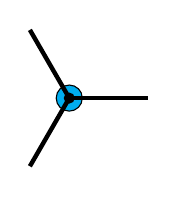
\begin{tikzpicture}
        \node at (0,0) [circle,draw,fill=cyan] (a) {};
        \fill (0,0) circle [radius=2pt,fill=black];
        \draw [ultra thick] (0,0) -- +(0:1cm);
        \draw [ultra thick] (0,0) -- +(120:1cm);
        \draw [ultra thick] (0,0) -- +(240:1cm);
    \end{tikzpicture}
    \caption{Three surface sides}
  \end{subfigure}
  \begin{subfigure}[c]{0.3\textwidth}
    \centering
    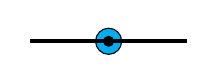
\begin{tikzpicture}
        \node at (0,0) [circle,draw,fill=cyan] (a) {};
        \fill (0,0) circle [radius=2pt,fill=black];
        \draw [ultra thick] (0,0) -- +(0:1cm);
        \draw [ultra thick] (0,0) -- +(180:1cm);
    \end{tikzpicture}
    \caption{Two surface sides}
  \end{subfigure}
  \caption{Examples of surface cardinality}
\end{figure}

For one of the sets surface cardinality of~$a$ is $3$ and for
another it is~$2$.

Now define \emph{shift special points}.

Let $I$ be an interval on~$\mathbb{R}$ (containing zero?)

A point~$a$ is \emph{shift special} if there exists a transformation
(that is a continuous function $f:I\times\mu\to\mu$ such that:
\begin{enumerate}
  \item $f(0)$ is identity. \fxwarning{Is this condition needed?}
  \item for every sufficiently small~$\epsilon>0$ we have $f(\epsilon,a)\in T$;
  \item there is $\epsilon>0$ such that for every $0<\epsilon'<\epsilon$ we have
    $f(\epsilon')$ being not continuous at~$a$ regarding complete funcoid
    defined by the function $x\mapsto\rsupfun{\mu}\{x\}\setminus T$.
\end{enumerate}

We may consider to additonally require that every~$f(\epsilon)$ is isomorphism
of funcoids.

\begin{example}
$T$~is disk $\setcond{(x,y,0)}{x^2+y^2\leq 1}$. $f$~is the contraction
$(\epsilon,v)\mapsto\frac{1}{1+\epsilon}v$. $a=(1,0,0)$.

In the usual topology~$f$ is continuous. In
$x\mapsto\rsupfun{\mu}\{x\}\setminus T$ we have the function
$\epsilon\mapsto f(\epsilon)$ not continuous at zero.
So~$a$ is a shift special point.
\end{example}

\begin{proof}
$f (0) (v) = v$. Thus $\langle f (0) \rangle (\rsupfun{\mu} \{ a
\} \setminus T) = \rsupfun{\mu} \{ a \} \setminus T$ intersects
the plane $Z = 0$. But $f (0, a)$

??
\end{proof}

\begin{question}
Can we exclude real numbers from the play?
\end{question}

\begin{question}
How cardinality special points, isomorphism special points and shift
special points are related with each others?
\end{question}

\begin{question}
How the number of surface sides is related with usual surface sides for
manifolds?
\url{https://en.wikipedia.org/wiki/Orientability#Orientability_of_manifolds}
\end{question}

\begin{rem}
Manifolds have no special points. (Prove!)
\end{rem}

Prove that $2$-manifold image which special points removed has the same number
of sides as the defined above.

Another way to define special points: A special point is a point
such that $T\sqcap\supfun{\mu}\{a\}$ is not isomorphic to
$T\sqcap\supfun{\mu}\{x\}$ for nearby points~$x$. Consider replacement
of isomorphism with injection, surjection, etc. here and above.

How many sides has in $\mathbb{R}^3$ a plane without one point?

Easy way to spot special points: They are boundary points in the
topology (or funcoid) induced on~$T$. Alternatively we can consider
points whose neighborhood in~$T$ is different (as non-isomorphic or
maybe non-injective or non-surjective or like this) than of nearby
points. Thus another way to remove special points: use interior funcoid.


% \printindex{}

\bibliographystyle{plain}
\bibliography{refs}

\end{document}
